\chapter{Cơ sở lý thuyết}
\paragraph{Giới thiệu} Chương này sẽ tập trung giới thiệu từ khái quát đến chi tiết về những đặc tính lý thuyết của Web Ngữ Nghĩa - Semantic Web, ngôn ngữ Ontology Web Language, ngôn ngữ Semantic Web Rule Language (SWRL) và tính nhất quán của ontology - ontology consistency. Đây là những nền tảng lý thuyết cơ bản nhất giúp chúng em xây dựng nên hệ thống phân loại.

%% ----------------------------------------------------------------
% 	Semantic Web
%% ----------------------------------------------------------------
\section{Semantic Web}
Nếu như chúng ta đã biết hệ thống Web mà chúng ta được sử dụng được gọi nôm na là Web 2.0 thì Semantic Web hay còn gọi là Web ngữ nghĩa được các nhà nghiên cứu kỳ vọng sẽ trở thành Web 3.0 trong tương lai gần với đặc trưng riêng biệt là phương thức liên kết dữ liệu (linked data) giữa các hệ thống hoặc các thực thể cho phép thể hiện được nhiều hơn, và rõ ràng hơn mối liên kết giữa các dữ liệu trên mạng lưới web toàn cầu. Cụ thể hơn, Semantic Web có khả năng chuyển đổi văn bản HTML của con người (human readable HTML documents) sang ngôn ngữ máy tính (machine readable documents), giúp cho máy tính làm được nhiều công việc suy nghĩ hơn cho con người \cite{semantic1}.
\\
Ngày nay, đa phần dữ liệu trên web được cung cấp dưới dạng trang web (web pages) - văn bản HTML được liên kết với nhau bằng các liên kết (hyperlinks). Cả người và máy tính đều có thể dễ dàng đọc hiểu những văn bản đó, tuy nhiên thay vì dễ dàng tìm kiếm những từ khoá trong trang web, máy tính lại gặp trở ngại khi chọn lọc những ý nghĩa trong các văn bản đó. Một trang web chứa rất nhiều thông tin, nhưng những thông tin đó không phải là những thông tin thô - mà chỉ là những văn bản HTML được xây dựng từ cơ sở dữ liệu. Vậy nên Semantic Web đã thay đổi hướng nhìn và đưa ra giải pháp cho vấn đề ở trên theo nhiều cách khác nhau :
\begin{itemize}
	\item Chuyển những trang web dữ liệu thành những tiến trình xử lý thông minh nhân tạo (giúp trang web phải “suy nghĩ” để xử lý giúp con người).
	\item Khuyến khích các công ty, các doanh nghiệp và các cá nhân trình bày dữ liệu tự do hơn, theo một quy chuẩn mở.
	\item Khuyến khích các doanh nghiệp sử dụng dữ liệu đã có sẵn trên web.
\end{itemize}
% 
\subsection{Semantic Web dựa trên giả định thế giới mở (Open World Assumption)} 
Với đặc điểm của thông tin trên Web là những thông tin luôn luôn cần được thêm vào hay chỉnh sửa (thông tin trên web cũng giống như kiến thức vì thế nó sẽ không bao giờ bị giới hạn) nên thay vì chọn tuân theo giả định thế giới đóng (Closed World Assumption - CWA), vốn đã tồn tại rất lâu trong các cơ sở dữ liệu quan hệ (SQL), các nhà nghiên cứu đã chọn giả định thế giới mở làm nguyên lý cho mọi lý thuyết và định nghĩa của Semantic Web. Một so sánh ngắn gọn giữa giả định Thế Giới Mở (Open World Assumption - OWA)\cite{OWA_0} được Semantic Web chấp nhận và giả định Thế Giới Đóng (CWA).
\begin{description}
	\item[Closed World Assumption] 
	Giả định Thế Giới Đóng (CWA) là giả định mà những điều không chắc hoặc không có cơ sở để chứng minh là \textbf{đúng} sẽ được chấp nhận là \textbf{sai}.
	\item[Open World Assumption]
	Giả định Thế Giới Mở (OWA) thì ngược lại, với những điều không chắc hoặc không có cơ sở để chứng minh là \textbf{đúng} sẽ được chấp nhận là \textbf{chưa biết}. 
	\item[Ví dụ]
	Xem xét một câu nói sau đây: "A là một công dân của nước Hoa Kỳ". Nếu có ai đó hỏi "A có phải là một công dân của Việt Nam hay không ?". Xét theo CWA, câu trả lời là \textit{không}, ngược lại với OWA thì câu trả lời là \textit{chưa biết}. 
\end{description}
%
\subsection{Các tiêu chuẩn và thành phần của Semantic Web}
Khái niệm "Semantic Web" thường được sử dụng cụ thể hơn nhằm chỉ đến những định dạng và công nghệ để hiện thực hóa nó. Việc tổ chức, tập hợp và phục hồi dữ liệu liên kết thực hiện được nhờ vào các công nghệ đặc tả chính thức về các khái niệm, định nghĩa và mối quan hệ trong một lĩnh vực tri thức được biết đến. Tất cả các công nghệ này đều được quy định thành một tiêu chuẩn của tổ chức World Wide Web Consortium (W3C) \cite{semantic2}. Các tiêu chuẩn được liệt kê dưới đây
\begin{figure}[h!]
	\centering
	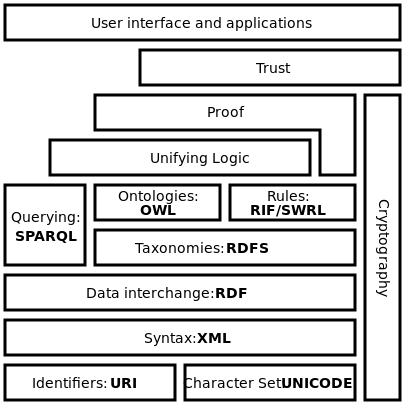
\includegraphics[width=110mm]{Figures/semantic_web_stack.png}
	\caption{The Semantic Web Stack \label{overflow}}
\end{figure}
\begin{itemize}
	\item \href{http://en.wikipedia.org/wiki/Resource\_Description\_Framework}{Resource Description Framework}, một phương thức chung để biểu diễn thông tin cho semantic web.
	\item \href{http://en.wikipedia.org/wiki/RDF_Schema}{RDF Schema}
	\item \href{http://en.wikipedia.org/wiki/Simple_Knowledge_Organization_System}{Simple Knowledge Organization System} (SKOS)
	\item \href{http://en.wikipedia.org/wiki/SPARQL}{SPARQL} - Ngôn ngữ truy vấn dữ liệu biểu diễn dưới dạng RDF.
	\item \href{http://en.wikipedia.org/wiki/Notation3}{Notation3}, thiết kế với tiêu chí hiểu được bởi con người.
	\item \href{http://en.wikipedia.org/wiki/N-Triples}{N-Triples}, một định dạng dùng để lưu và truyền dữ liệu.
	\item \href{http://en.wikipedia.org/wiki/Turtle_(syntax)}{Turtle} (Terse RDF Triple Language)
	\item \href{http://en.wikipedia.org/wiki/Web_Ontology_Language}{Web Ontology Language} (OWL), một họ các ngôn ngữ biểu diễn tri thức.
	\item \href{}{Rule Interchange Format} (RIF), một framework chung của các ngôn ngữ điều luật web hỗ trợ chuyển đổi nhiều điều luật khác nhau trên web.
\end{itemize}

Hình Semantic Web Stack \cite{semantic3} miêu tả kiến trúc của Semantic Web:

\begin{enumerate}
	\item XML cung cấp một cú pháp cơ bản nhất cho nội dung bên trong tài liệu, và không có liên quan gì đến mặt ngữ nghĩa mà nội dụng nó chứa. XML không phải là một thành phần cần thiết trong các công nghệ Semantic Web trong hầu hết các trường hợp, tồn tại cú pháp thay thế khác như Turle \textsuperscript{*}. 
	\item XML Schema là một ngôn ngữ dùng để cung cấp và hạn chế cấu trúc nội dung của các thành phần nằm trong tài liệu XML, nói cách khác nó giúp chúng ta đáng giá nội dung mà tài liệu đó chứa là gì. Ví dụ: OWL/XML vs. RDF/XML
	\item RDF \cite{rdf} là một ngôn ngữ đơn giản dùng để diễn tả các mô hình dữ liệu (ở đây muốn chỉ đến các nguồn dữ liệu web) và mối quan hệ của chúng. Một mô hình dựa theo RDF có thể được biểu diễn bằng nhiều cú pháp khác nhau, vd: RDF/XML, N3, Turtle và RDFa. Có thể nói RDF chính là thành phần cơ bản và quan trọng nhất của Semantic Web.
	\item RDF Schema \cite{rdfs} mở rộng RDF và là từ vựng để đặc tả các thuộc tính và lớp trong các tài nguyên dựa trên RDF, với ngữ nghĩa dựa trên các việc tạo ra nhiều phân cấp lớp và thuộc tính.
	\item OWL thêm nhiều từ vựng hơn để diễn các thuộc tính và lớp, và điểm quan trọng của nó là thêm các từ vựng để đặc tả mối quan hệ giữa các lớp với nhau. Ví dụ: ranh giới riêng biệt giữa các lớp với nhau (disjointness), các quy định với số lượng (cardinality), cung cấp nhiều loại dữ liệu cho các thuộc tính, và các đặc tính của các thuộc tính (đối xứng/ bất đối xứng, và các lớp liệt kê, ...).
	\item SPARQL là một giao thức và ngôn ngữ truy vấn dữ liệu dành cho tài nguyên của Semantic Web.
	\item RIF (W3C Rule Interchange Format) là một ngôn ngữ XML để biểu diễn điều luật web mà máy tính có thể thực thi.
\end{enumerate}
{\let\thefootnote\relax\footnotetext{*\textit{
			Turtle: http://en.wikipedia.org/wiki/Turtle\_(syntax)}}
}
%% ----------------------------------------------------------------
% 	Kết thúc Semantic Web
%% ----------------------------------------------------------------
% 	Ontology Web Language 
%% ----------------------------------------------------------------
\section{Ontology Web Language 2}
Được giới thiệu trong các thành phần của Web Ngữ nghĩa, nhiệm vụ của Ontology Web Language (OWL) là đem lại đặc tính ngữ nghĩa cho Semantic Web. OWL được tổ chức W3C khuyến khích sử dụng vì những thành phần từ vựng mới của nó giúp đặc tả các thực thể trong một lĩnh vực nào đó hiệu quá hơn so với RDFS hay RDF. Phiên bản OWL hiện thời là phiên bản 2 \cite{owl2}. Về mặt lý thuyết, OWL là một ngôn ngữ ontology tuân theo Description Logic (DL) $SROIQ_{(D)}$ \cite{DL}, với ưu điểm là ngoài  khả năng đặc tả vừa nêu, nó còn biểu diễn được những suy luận được suy ra từ những đặc tả được khai báo.
\subsection{Đặc điểm tổng quan}
\begin{figure}[h!]
	\centering
	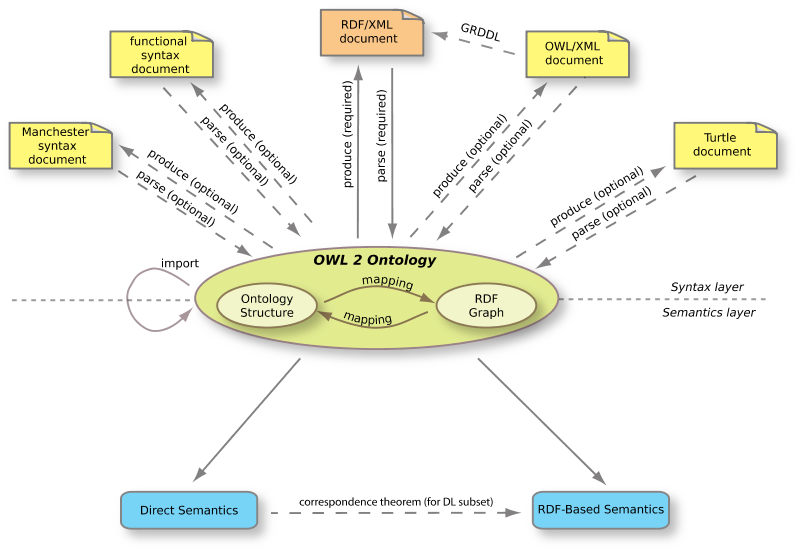
\includegraphics[width=120mm]{Figures/owl2structure.png}
	\caption{Cấu trúc của OWL 2\label{overflow}}
\end{figure}
Hình trên cho chúng ta cái nhìn tổng quan về các định dạng file, các loại cú pháp và các khả năng serialization thành RDF Graph của Ontology. Chúng ta thấy trong hình, hình eclipse ở giữa thể hiện khái niệm trừu tượng của một ontology, có thể hiểu là một cấu trúc trừu tượng hay một đồ thi RDF. Chúng ta có thể dùng nhiều cú pháp để biểu diễn ontology và định dạng chúng dưới dạng file khác nhau (Syntex layer trong hình), các định dạng và cú pháp này hoàn toàn có thể chuyển đổi qua lại với nhau. Lớp ngữ nghĩa trong hình (semantic layer) cho thấy ngữ nghĩa được quy định theo 2 tiêu chuẩn kỹ thuật khác nhau là Direct Semantics và RDF-Based Semantics.
\subsubsection{Ontologies}
Bất kì ontology OWL2 nào đều có thể được định dạng như một đồ thị RDF (RDF Graph). Mối quan hệ giữa 2 cách này được quy định bởi các tài liệu Mapping to RDF Graphs document [\href{http://www.w3.org/TR/owl2-overview/#ref-owl-2-rdf-mapping}{OWL 2 RDF Mapping}] \cite{mapping_rdf_graph}, trong tài liệu này định nghĩa rất rõ ràng một bảng map từ định dạng cấu trúc của ontology qua đồ thị RDF, và ngược lại. 
\subsubsection{Cú pháp}
Trong thực tế, một cú pháp cụ thể rất cần thiết để lưu trữ các OWL2 Ontologies và để trao đổi chúng giữa các công cụ và ứng dụng khác nhau. Cú pháp đầu tiên có khả năng hoán đổi là RDF/XML [\href{http://www.w3.org/TR/owl2-overview/#ref-rdf-syntax}{RDF Syntax}] \cite{rdfxml}. Ngoài RDF/XML có khả năng cung cấp khả năng tương tác giữa nhiều ứng dụng OWl2 khác nhau, các loại cú pháp khác đều có thể được sử dụng. Dưới đây là bảng so sánh và liệt kê các cú pháp.
\begin{table}[H]
	\begin{tabular}{ |p{3cm}|p{4cm}|p{2cm}|p{4cm}|}
		\hline
		Tên cú pháp & Mô tả & Trạng thái & Mục đích sử dụng\\
		\hline
		RDF/XML & Mapping to RDF Graphs \cite{mapping_rdf_graph} \cite{rdfxml} & Bắt buộc & Hoán đổi được ( có thể viết và đọc được bằng nhiều phần mềm OWL2)
		\\
		\hline
		OWL/XML & XML Serialization \cite{owlxml} & Tùy chọn & Xử lý dễ dàng hơn bằng công cụ XML.
		\\
		\hline
		Functional Syntax & Structural Specification \cite{func_syntax} & Tùy chọn & Dễ đọc và hiểu được.
		\\
		\hline
		Manchester Syntax & Manchester Syntax \cite{man_syntax} & Tùy chọn & Có ưu thế hơn để đọc/ghi DL Ontologies
		\\
		\hline
		Turtle & Mapping to RDF Graphs \cite{mapping_rdf_graph} & Tùy chọn, không được công nhận chính thức & Có ưu thế để đọc/ghi RDF triples
		\\
		\hline
	\end{tabular}
	\caption{Bảng so sánh các cú pháp của OWL2\label{overflow}}
\end{table}
\subsection{Một số ví dụ của các syntax}

\textbf{Functional Syntax}
\begin{verbatim}
Declaration(Class (Grass))) # Khai báo lớp
Declaration(ObjectProperty (canEat))  # Khái báo thuộc tính
SubClassOf(Cow Animal)  # Khai báo lớp con
\end{verbatim}

\textbf{RDF/XML Syntax}
\begin{verbatim}
T(Animal) rdf:type owl:Class
T(canEat) rdf:type owl:ObjectProperty
T(Cow) rdfs:subClassOf T(Animal) 
\end{verbatim}


\textbf{OWL/XML Syntax}
\begin{verbatim}
<Declaration>
<Class IRI="#Animal"/> // Khai báo lớp
</Declaration>
<Declaration>
<ObjectProperty IRI="#canEat"/> // Khai báo thuộc tính
</Declaration>
<SubClassOf>
<Class IRI="#Cow"/>
<Class IRI="#Animal"/>  // Khai báo lớp con
</SubClassOf>
\end{verbatim}

\textbf{Manchester Syntax}
\begin{verbatim}
Class: Cow  # Khái báo lơp chung với lớp con
	SubClassOf: Animal 
	SubClassOf: canEat some Grass
\end{verbatim}


\subsection{Các thành phần chi tiết của một OWL 2 ontology}

\subsubsection{Ontology IRI và Version IRI}
Mỗi ontology đều có thế gồm \textit{một ontology IRI} \cite{iri} \textsuperscript{*} (Internationalized Resource Identifier), dùng để định danh cho ontology. Nếu một ontology có một ontology IRI, thì ontology này có thể có thêm một version IRI, dùng để xác định phiên bản cho ontology này. Version IRI có thể trùng hoặc không cần thiết phải trùng với ontology IRI. Một ontology không có ontology IRI thì không có version IRI.
Dưới đây là những quy ước chọn ontology IRIs và version IRIs trong OWL2. Những đặc điểm kỹ thuật này không cung cấp cơ chế nào để làm chúng phải được tuân theo trên toàn hệ thống web. Tuy nghiên, những công cụ hay ứng dụng OWl2 \textit{nên} sử dụng những quy ước này để dễ dàng tìm ra lỗi trong những ontology mà chúng xử lý.
{\let\thefootnote\relax\footnotetext{*\textit{
			Internationalized Resource Identifier: giao thức bổ sung cho Uniform Resource Universal Character Set (Unicode/ISO 10646).}}
}
\begin{itemize}
	\item Nếu một ontology có một ontology IRI nhưng không có version IRI, thì \textit{không nên tồn tại} một ontology với trùng ontology IRI vừa đặt.
	\item Nếu một ontology có một ontology IRI và một version IRI, thì \textit{không nên tồn tai} một ontology khác với trùng ontology IRI và version IRI vừa đặt.
	\item Tất cả các cách kết hợp khác của ontology IRI và version IRI không cần đòi hỏi tính duy nhất (unique). Như vậy 2 ontologies khác nhau có thể không có ontology IRI và version IRI; tương tự, một ontology chưa một ontology IRI có thể cùng tồn tại cùng với một ontology khác có cùng ontology IRI vừa đặt \textbf{và} các version IRI của các ontologies này \textbf{phải} khác nhau.
\end{itemize}
Ontology IRI và các version IRI kết hợp với nhau giúp định danh một phiên bản cụ thể của của ontology từ một bộ chứa tất cả các phiên bản của một ontology cụ thể nào đó được định danh chung bằng ontology IRI. Trong mỗi bộ ontology như vậy, sẽ có chính xác một ontology được dùng như một ontology hiện hành - khi dùng ontology IRI để truy vấn ontology mà không đề cập đến version IRI, mặc định ontology có verison IRI hiện hành sẽ được trả về.


\subsubsection{Thực thể, trực nghĩa và cá thể ẩn danh - Entities, Literals and Anonymous Individuals}
Các thực thể (entities) là thành phần cơ bản nhất của OWL2 Ontology, chúng định nghĩa các từ vựng - cụ thể là những đặt tên ra các khái niệm (named term) - của một ontology. Bên cạnh các thực thể, OWL 2 ontologies thường có thêm các trực nghĩa (literals), như strings hay integers.
\begin{figure}[ht!]
	\centering
	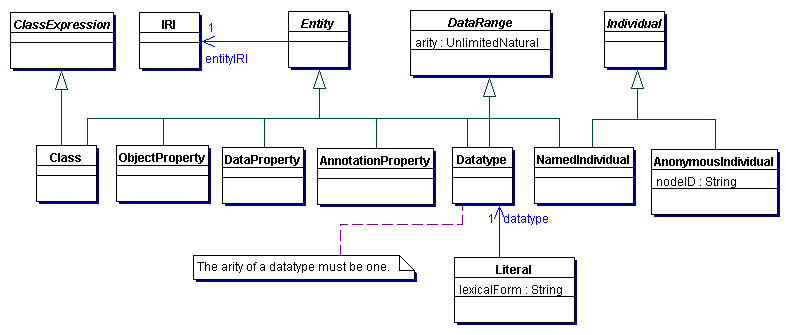
\includegraphics[width=150mm, height=80mm]{Figures/entities.png}
	\caption{Entities, Literals, Anonymous Individuals trong OWL2 \label{overflow}}
\end{figure}
\\
Cấu trúc của các thực thể và trực nghĩa trong OWL 2 được thể hiện trong hình bên. Các lớp (classes), kiểu dữ liệu (datatypes), thuộc tính đối tượng (object properties), thuộc tính dữ liệu (data properties), thuộc tính chú thích và các cá thể có tên đều được gọi chung là các thực thể (entities), tất cả chúng được được định danh bằng một IRI duy nhất. 
\begin{itemize}
	\item Lớp (class) đại diện cho một tập gồm nhiều cá thể(individuals).
	\item Kiểu dữ liệu (datatype) là một tập của các trực nghĩa như strings hoặc integers.
	\item Thuộc tính đối tượng và dữ liệu (object \& data property) được sử dụng để biểu diễn các mối quan hệ giữa các cá thể với cá thể khác và giữa cá thể với trực nghĩa (literal) trong một lĩnh vực (domain) nào đó.
	\item Thuộc tính chú thích (annotation) được dùng để đưa thêm những thông tin không có tính ngữ nghĩa(non-logical) như các chú thích, giải nghĩa, ngôn ngữ gắn với ontologies, các phát biểu/tiên đề (axioms) và các thực thể.
	\item  Các cá thể có tên có thể được dùng để biểu diễn một đối tượng cụ thể từ một lớp nào đó.
\end{itemize}
Bên cạnh các cá thể có tên, OWL2 còn cung cấp một khái niệm gọi là các cá thể ẩn danh (anonymous individuals) - là cá thể tương tự với các node trống (blank nodes) trong RDF Concept \cite{rdf_concept} và được truy xuất ngay bên trong ontology mà chúng được sử dụng. Cuối cùng, OWL 2 cung cấp thêm cho cac trực nghĩa (literals), một dạng dữ liệu string gọi là định dạng nghĩa bằng từ ngữ (lexical form) và một dạng dữ liệu để chỉ dẫn cách ontology có thể hiểu chuỗi này.
% Classes 
\paragraph{Lớp (Classes)}
Lớp được hiểu như tập hợp các cá thể. Hai lớp với IRIs \textit{owl:Nothing} và \textit{owl:Thing} là các lớp được định nghĩa sẵn trong OWL2 với ý nghĩa như sau:
\begin{itemize}
	\item \textbf{owl:Thing} là tập hợp gồm tất cả các cá thể.
	\item \textbf{owl:Nothing} là tập hợp rỗng.
\end{itemize}
Không nên sử dụng 2 định nghĩa trên để gán cho bất kì lớp nào trong OWL 2 DL Ontology. 
Ví dụ:
\begin{verbatim}
SubClassOf( a:Child a:Person) 
\end{verbatim}
\textbf{Giải thích:} Mỗi đứa trẻ đều là một người.

% Datatypes
\paragraph{Kiểu dữ liệu (datatypes)}
Kiểu dữ liệu là thực thể được xem như tập hợp của các giá trị dữ liệu. Như vậy, kiểu dữ liệu cũng tương tự lớp, khác biệt chính là thay vì chứa các cá thể (individuals) như lớp thì lại chứa các giá trị dữ liệu như strings, numbers,... Kiểu dữ liệu có thể được dùng tạo ra các dữ liệu giới hạn (datarange). Ví dụ kiểu dữ liệu \textit{xsd:positiveInteger} đại diện cho tập hợp gồm tất cả các số nguyên dương. Nó được sử dụng để quy định kiểu dữ liệu mà thuộc tính \textit{hasAge} có thể chấp nhận:

\begin{verbatim}
DataPropertyRange( a:hasAge xsd:positiveInteger) 
\end{verbatim}

\textbf{Giải thích:} thuộc tính dữ liệu a:hasAge chỉ được phép là các số nguyên dương.

% Object Properties
\paragraph{Thuộc tính đối tượng (object properties)} 
Thuộc tính đối tượng kết nối các cặp cá thể - tạo ra mối liên hệ (relationship) giữa các cá thể. Tương tự như lớp cũng có 2 thuộc tính đối tượng được định nghĩa sẵn trong OWL 2 với ý nghĩa như sau:
\begin{itemize}
	\item \textbf{owl:topObjectProperty} kết nối tất cả các cặp cá thể có thể kết nối.
	\item \textbf{owl:bottomObjectProperty} không kết nối bất kì cặp cá thể nào. 
\end{itemize}
Không nên sử dụng 2 định nghĩa trên để gán cho bất kỳ thuộc tính đối tượng nào trong OWL 2 DL Ontology. Ví dụ:
\begin{verbatim}
ObjectPropertyAssertion( a:parentOf a:Peter a:Chris)  
\end{verbatim}
\textbf{Giải thích:} Peter là ba mẹ của Chris. Thuộc tính đối tượng \textit{a:parentOf} được dùng để nói lên mối quan hệ giữa các cá thể trong ví dụ trên.

% Data Properties
\paragraph{Thuộc tính dữ liệu (data properties)}
Thuộc tính dữ liệu liên kết các cá thể với các trực nghĩa. Trong một vài hệ thống biểu diễn tri thức, thuộc tính dữ liệu chức năng được gọi là thuộc tính.
Hai định nghĩa sẵn \textit{owl:topDataProperty} và \textit{owl:bottomDataProperty} có ý nghĩa như sau :
\begin{itemize}
	\item \textbf{owl:topDataProperty} liên kết tất cả cá thể với tất cả các trực nghĩa.
	\item \textbf{owl:bottomDataProperty} không liên kết bất kì cá thể với trực nghĩa nào.
\end{itemize}
Tương tự lớp và thuộc tính đối tượng, 2 phát biểu \textit{top} và \textit{bottom} trên cũng không nên được sử dụng để gán cho bất kì thuộc tính dữ liệu nào. Mỗi thuộc tính dữ liệu \textit{a:hasName} chứa tên đầy đủ của mỗi người. Ví dụ nó có thể được sử dụng như trong phát biểu sau:

\begin{verbatim}
DataPropertyAssertion( a:hasName a:Steve "Steve Job") 
\end{verbatim}

\textbf{Giải thích:} Tên của Steve là "Steve Job".

% Individuals
\paragraph{Cá thể (Individuals)}
Cá thể trong OWL2 là một đối tượng cụ thể thuộc một tập/lớp (domain/class). Có 2 dạng cá thể trong cú pháp OWL2. \textit{Cá thể có tên} được khai báo tên một cách rõ ràng để có thể sử dụng trong bất kì ontology nào bằng cách truy vấn tới IRI có chứa tên của nó. Ngược lại, cá thể ẩn danh (Anonymous Individuals) không có tên gọi toàn cục và chỉ truy vấn được trong nội bộ của ontology chứa chúng.

% Named Individuals
\subparagraph{Cá thể có tên (Named Individuals)} được định danh bằng một IRI. Vì vậy, nên cá thể có tên cũng là một thực thể (entity) tương tự lớp, thuộc tính và kiểu dữ liệu. Ví dụ khai báo một các thể thuộc 1 lớp:


\begin{verbatim}
ClassAssertion( a:Person a:Peter)
\end{verbatim}


\textbf{Giải thích:} Peter là một người.

% Anonymous Individuals
\subparagraph{Cá thể ẩn danh (Anonymous Individuals)} Nếu cần một cá thể chỉ sử dụng ở nội bộ ontology, chúng ta có thể sử dụng cá thể ẩn danh, được định danh bằng một node ID cục bộ thay vì sử dụng IRI toàn cục. Cá thể ẩn danh tương tự như một node rỗng trong đồ thị RDF \cite{rdf_concept}. Ví dụ khai báo thuộc tính đối tượng giữa cá thể ẩn danh với cá thể có tên:

\begin{verbatim}
ObjectPropertyAssertion( a:liveAt a:Peter _:a1)
ObjectPropertyAssertion( a:city _:a1 a:HCM)
ObjectPropertyAssertion( a:district _:a1 a:ThuDuc)
\end{verbatim}

\textbf{Giải thích:} Peter sống ở một địa chỉ nào đó (chưa biết). Mà địa chỉ chưa biết này nằm trong thành phố Hồ Chí Minh và nằm trong quận Thủ Đức.

% Literals
\paragraph{Trực nghĩa (Literals)}
Trực nghĩa biểu diễn các giá trị dữ liệu như chuỗi và số nguyên. Mỗi trực nghĩa gồm một chuỗi định dạng được định nghĩa bới người dùng (lexical form), và một kiểu dữ liệu được hỗ trợ bởi OWL2 \cite{owl2spec} . Một trực nghĩa gồm một chuỗi định dạng \textit{"abc"} và một kiểu dữ liệu (Datatype) định danh bởi IRI \textit{datatypeIRI} được định nghĩa như sau \verb|"abc"^^datatypeIRI|. Thêm nữa, các trực nghĩa mà kiểu dữ liệu của chúng là \textit{rdf:PlainLiteral} có thể được viết tắt trong functional-syntax của OWL2 ghi lại trong tài liệu thành dạng trực nghĩa rỗng RDF \cite{rdf_concept}. Cú pháp viết tắt này chỉ đơn giản là một định dạng ngắn gọn hơn, chúng không có ảnh hưởng đến ý nghĩa của khai báo trực nghĩa. Viết tắt chủ yếu là để phục vụ cho việc parsing:
\begin{itemize}
	\item Trực nghĩa dạng \verb|"abc@"^^rdf:PlainLiteral| được viết tắt thành \verb|"abc"|.
	\item Trực nghĩa dạng \verb|"abc@langTag"^^rdf:PlainLiteral| trong đó \textit{"langTag"} không rỗng được viết tắt thành \verb|"abc"@langTag|.
\end{itemize}
Một số ví dụ:
\begin{verbatim}
"1"^^xsd:integer  // trực nghĩa biểu diễn số nguyên dương 1
"abc"^^xsd:string // trực nghĩa biểu diễn chuỗi "abc"
\end{verbatim}

% Entity Declarations and Typing
\paragraph{Khai báo thực thể}
Mỗi IRI \textit{I} được sử dụng trong OWL 2 ontology \textit{O} cần được khai báo để sử dụng. Phát biểu khai báo một thực thể \textit{I} nhằm đảm bảo rằng \textit{O} phải chứa \textit{I}. Hai mục tiêu của phát biểu này:
\begin{itemize}
	\item Khẳng định sự tồn tại trong \textit{I} trong \textit{O}
	\item Khai báo gắn với loại của thực thể \textit{I} - phân loại xem \textit{I} có phải là một lớp, một kiểu dữ liệu, một thuộc tính đối tượng, một thuộc tính dữ liệu, một đặt tính chú thích hay một cá thể.
\end{itemize}
Bối cảnh sử dụng khái báo \textbf{Declaration} thường gắn liền với chức năng \textit{Add New Class/Property/Datatype} trong một Ontology Editor nào đó. Ví dụ:
\begin{verbatim}
Declaration( Class( a:Person ) )
Declaration( NamedIndividual( a:Peter ) )
\end{verbatim}

% Property Expression
\subsubsection{Mô tả thuộc tính (Property Expression)}
Các thuộc tính được sử dụng trong OWL 2 để tạo ra các mô tả thuộc tính.

% Object Property Expression
\paragraph{Mô tả thuộc tính đối tượng (Object Property Expression)}
Thuộc tính đối tượng được sử dụng trong OWL 2 để tạo thành các mô tả thuộc tính đối tượng (object property expression), diễn tả các mối quan hệ giữa các cặp cá thể. Chúng được diễn giải trong tài liệu cấu trúc chi tiết của OWL 2 như trong hình sau.
\begin{figure}[h!]
	\centering
	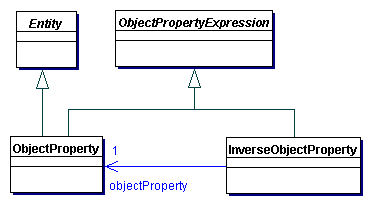
\includegraphics[width=120mm]{Figures/object_property_expression.png}
	\caption{Mô tả thuộc tính đối tượng OWL 2\label{overflow}}
\end{figure}
Như được thể hiện trong hình, OWL 2 hỗ trợ 2 loại mô tả thuộc tính đối tượng. Thuộc tính đối tượng là dạng đơn giản của mô tả thuộc tính đối tượng, thuộc tính đối tượng nghịch đảo (inverse object properties) cho phép thể hiện các mối quan hệ 2 chiều giữa biểu hiện các mô tả lớp (class expression) và các phát biểu (axiom).
\\ \textbf{Mô tả thuộc tính đối tượng nghịch đảo}

\begin{verbatim}
ObjectPropertyAssertion( a:fatherOf a:Peter a:Steve) 
// Peter là ba của Steve
\end{verbatim}}
Với phát biểu trên, ontology sẽ hiểu \textit{a:Steve} liên kết với \textit{a:Peter} qua một thuộc tính nghịch đảo của \textit{a:fatherOf} là \textit{ObjectInverseOf( a:fatherOf)}. Chúng ta cũng có thể khai báo tường minh nghịch đảo của \textit{a:fatherOf} là \textit{a:childOf} bằng phát biểu  \textit{InverseObjectProperties( a:fatherO a:childOf )}.

% Data Property Expression
\paragraph{Mô tả thuộc tính dữ liệu (Data Property Expression)}
Tương đương với biểu hiện thuộc tính đối tượng, trong tài liệu cấu trúc chi tiết của OWL2 cũng giới thiệu định nghĩa mô tả thuộc tính dữ liệu (data property expressions), nhằm biểu diễn mối quan hệ giữa một cá thể và một trực nghĩa. Cấu trúc của mô tả thuộc tính dữ liệu thể hiện trong hình bên. Như chúng ta thấy thuộc tính dữ liệu (data property) cũng chính là 1 mô tả thuộc tính dữ liệu (data property expression), cấu trúc như vậy được xây dựng nhằm tạo thuận lợi cho nhu cầu mở rộng sau này nếu có.
\begin{figure}[h!]
	\centering
	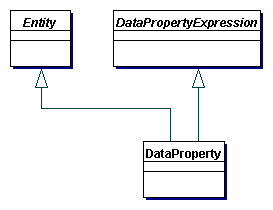
\includegraphics[width=110mm]{Figures/data_property_expression.png}
	\caption{Cấu trúc của mô tả thuộc tính dữ liệu OWL 2\label{overflow}}
\end{figure}

%Data ranges
\subsubsection{Miền dữ liệu (Data Range)}
Kiểu dữ liệu như\textit{xsd:string} hoặc \textit{xsd:integer} và trực nghĩa \verb|"1"^^xsd:integer| được dùng để biểu diễn miền dữ liệu - tập hợp danh sách có thứ tự (tuples) của các trực nghĩa, mà mỗi phần tử trong danh sách này chỉ chứa một trực nghĩa duy nhất để định nghĩa chính nó. Miền dữ liệu được dùng để tạo ra ràng buộc (hay những dữ liệu hợp lệ) cho thuộc tính dữ liệu. Cấu trúc của miền dữ liệu trong OWL 2 được mô tả trong hình. Thành phần đơn giản của miền dữ liệu chính là kiểu dữ liệu : một kiểu dữ liệu (Datatype) cũng chính là một miền dữ liệu (Data Range).
\begin{figure}[h!]
	\centering
	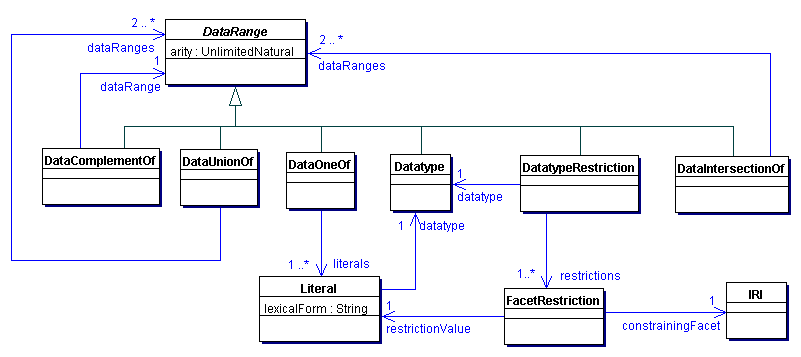
\includegraphics[width=150mm, height=80mm]{Figures/datarange.png}
	\caption{Cấu trúc miền dữ liệu (data range) quy định theo OWL 2\label{overflow}}
\end{figure}

% DataIntersectionOf
\paragraph{Giao của các miền dữ liệu (Intersection of Data Ranges)}
Giao của miền dữ liệu \textit{DataIntersectionOf(} $DR_{1} ... DR_{n}$ \textit{)}  chứa tất cả các danh sách của các trực nghĩa nằng trong $DR_{i}$ với $1 <= i <= n$. Tất cả miền dữ liệu $DR_{i}$ phải có cùng số lượng tham số, và cũng phải có cùng số lượng số kết quả trả về. Ví dụ về miền dữ liệu chỉ chứa số 0:
\begin{verbatim}
DataIntersectionOf( xsd:nonNegativeInteger xsd:nonPositiveInteger )
\end{verbatim}

% DataUnionOf
\paragraph{Hội của các miền dữ liệu (Union of Data Ranges)}
Điều kiện về số lượng tham số và số lượng kết quả trả về của từng $DR_{i}$ với điều kiện $1 <= i <= n$ phải giống nhau. Cú pháp \textit{DataIntersectionOf( $DR_{1} ... DR_{n}$ )}. Ví dụ về việc miền dữ liệu chứa tất cả các chuỗi và số nguyên:
\begin{verbatim}
DataUnionOf( xsd:string xsd:integer )
\end{verbatim}

% DataComplementOf
\paragraph{Phủ định của miền dữ liệu (Complement of Data Ranges)}
Cú pháp \textit{DataComplementOf( DR )} chứa tất cả các miền dữ liệu còn lại trong miền dữ liệu \textit{DR}. Yêu câu số lượng tham số và kết quả phải bằng \textit{DR}
\begin{verbatim}
DataComplementOf( xsd:positiveInteger )
\end{verbatim}
\textbf{Giải thích:} miền dữ liệu trên chứa tất cả số nguyên âm, số 0; và chứa tất cả chuỗi (strings) vì chuỗi không phải số nguyên dương.

% DataOneOf
\paragraph{Liệt kê trực nghĩa (Enumeration Of Literals)}
Một danh sách liệt kê các trực nghĩa (literals) với cú pháp \textit{DataOneOf(} $lt_{1} ... lt_{n}$ \textit{)},  $lt_{i}$ với $1 <= i <= n$.  Miễn dữ liệu chỉ áp dụng lên một trực nghĩa nằm trong danh sách (\textit{"oneOf"}). Ví dụ khai báo miền dữ liệu cho thuộc tính dữ liệu \textit{canMoveOnOrIn} chỉ có thể là một trong 4 giá trị chuỗi \textit{"OnRoadOrOffRoad"}, \textit{"Rail"}, \textit{"Sky"} và \textit{"Water"}.
\begin{verbatim}
DataPropertyRange(:canMoveOnOrIn 
DataOneOf("OnRoadOrOffRoad" "Rail" "Sky" "Water"))
\end{verbatim}

% Datatype Restrictions
\paragraph{Ràng buộc cho kiểu dữ liệu (Datatype Restrictions)}
Một ràng buộc cho kiểu dữ liệu (hay một tập các giá trị hợp lệ của kiễu dữ liệu) \textit{DatatypeRestriction(} $DT$ $F_{1}$ $lt_{1}$ ... $F_{n}$ $lt_{n}$ \textit{ )} gồm một kiểu dữ liệu đơn (unary datatype) $DT$ và $n$ cặp $($ $F_{i}$, $lt_{i}$ $)$. Vùng dữ liệu hợp lệ được tính ra bằng cách hạn chế vùng giá trị của $DT$ và lấy giao tất cả các cặp $(F_{i}$, $v_{i}$ $)$ trong đó $v_{i}$ là giá trị dữ liệu của trực nghĩa $lt_{i}$. Ví dụ miền dữ liệu sau chỉ gồm đúng các số 5,6,7,8,9:
\begin{verbatim}
DatatypeRestriction( xsd:integer 
xsd:minInclusive "5"^^xsd:integer xsd:maxExclusive "10"^^xsd:integer )
\end{verbatim}

% Class Expressions
\subsubsection{Mô tả lớp (Class Expression)}
Trong OWL2, các lớp và mô tả thuộc tính (property expressions) được sử dụng để xây dựng nên các mô tả lớp, hay chúng được gọi là các miêu tả hoặc trong thuật ngữ của Description Logic chúng được gọi là \textit{những khái niệm phức tạp}. Các mô tả lớp 
biểu diễn tập hợp các cá thể bằng cách chính thức đặt ra các điều kiện quy định cho các thuộc tính của các cá thể này; cá thể nào có những thuộc tính phù hợp hay thỏa những quy định đó được xem là một thành viên của mô tả lớp đang xét. Có 5 dạng mô tả lớp chính. Sau đây chúng em xin được trình bày 3 dạng mô tả lớp.
% Propositional Connectives and Enumeration of Individuals
\paragraph{Các mệnh đề logic và liệt kê cá thể}
\begin{figure}[h]
	\centering
	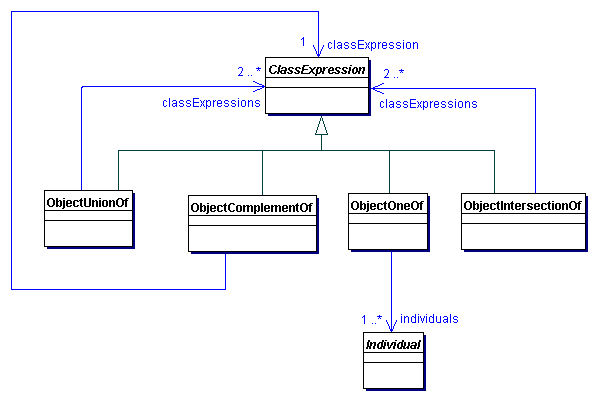
\includegraphics[width=150mm]{Figures/ce_0.png}
	\caption{Mô tả lớp trong OWL 2\label{overflow}}
\end{figure}
OWL2 cho phép liệt kê các cá thể của một lớp, khai báo các mệnh đề logic như trong hình sau. Các khai báo \textit{ObjectIntersectionOf}, \textit{ObjectUnionOf}, và \textit{ObjectComplementOf} cho phép thực hiện các phép toán luân lý (and ,or, not) trên những mô tả lớp. \textit{ObjectOneOf} quy định chính xác những cá thể cho mô tả lớp đang khai báo.

%% Intersection of Class Expressions
\subparagraph{Intersection of Class Expressions} Tập giao của các mô tả lớp \textit{ObjectIntersectionOf(} $CE_{1}$ ... $CE_{n}$ \textit{)} gồm tất cả các cá thể là thành viên của tất cả các mô tả lớp $CE_{i}$ với $1<=i<=n$. Ví dụ: 
\begin{verbatim}
ClassAssertion(a:Engineer a:Peter)  // Peter là kĩ sư.
ClassAssertion(a:Teacher a:Peter) // Peter là giáo viên.
\end{verbatim}
\textbf{Giải thích: } với khai báo như trên, một hàm ý sẽ được suy ra mà không cần khai báo đó là \textit{Peter vừa là giáo viên vừa là kĩ sư} hay tương đương với phát biểu \textit{ObjectIntersectionOf( a:Engineer a:Teacher )}. 

%% Union of Class Expressions
\subparagraph{Union of Class Expressions} Tập hội của lớp \textit{ObjectUnionOf(} $CE_{1}$ ... $CE_{n}$ \textit{)} chức tất cả các cá thể là thành viên của của ít nhất một mô tả lớp $CE_{i}$ với $1<=i<=n$. Ví dụ:
\begin{verbatim}
ClassAssertion( a:Man a:Peter )	 // Peter là nam
ClassAssertion( a:Woman a:Lois ) // Lois là nữ
\end{verbatim}
\textbf{Giải thích: } với khai báo như trên, một hàm ý sẽ được suy ra mà không cần khai báo đó là \textit{cả Peter và Lois đều thuộc lớp nam hoặc nữ} hay tương đương với phát biểu O\textit{bjectUnionOf( a:Man a:Woman )}.

%% Complement of Class Expressions
\subparagraph{Complement of Class Expressions} Phủ định của một mô tả lớp chứa tất cả các phần tử không thuộc mô tả lớp đó. Cú pháp \textit{ObjectComplementOf(CE)}. Ví dụ:
\begin{verbatim}
DisjointClasses( a:Man a:Woman) 
// Không có cá thể nào vừa làm nam vừa là nữ
ClassAssertion( a:Woman a:Lois) 
// Lois là nữ
\end{verbatim}
\textbf{Giải thích:} Vì \textit{Lois} là nữa và không có cá thể nào vừa là nam vừa là nữ nên \textit{Lois} thuộc lớp \textit{không phải nam} tương đương với phát biểu \textit{ObjectComplementOf( a:Man )}.

\subparagraph{Enumeration of Individuals} Liệt kê các cá thể \textit{ObjectOneOf(} $a_{1}$ ... $a_{n}$ \textit{)} chứa duy nhất một cá thể $a_{i}$ với $1<=i<=n$. 

% Object Property Restrictions 
\paragraph{Ràng buộc theo thuộc tính đối tượng (Object Property Restrictions)}
\begin{figure}[h]
	\centering
	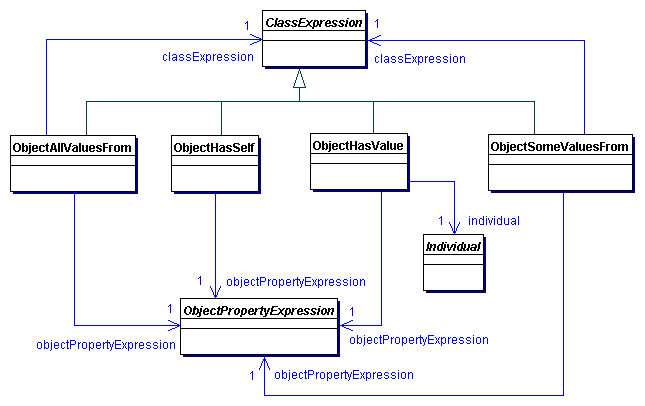
\includegraphics[width=150mm]{Figures/ce_1.png}
	\caption{Object Property Restrictions trong OWL 2\label{overflow}}
\end{figure}
Các mô tả lớp trong OWL 2 có thể được tạo ra bằng cách kết hợp chúng với các thuộc tính đối tượng bằng phát biểu như trong hình.
\paragraph{Existential Quantification} Một mô tả lớp \textit{ObjectSomeValueFrom( OPE CE )} thể hiện mối quan hệ giữa những cá thể được kết nối bởi mô tả thuộc tính đối tượng \textit{OPE} đến \textbf{ít nhất một} cá thể thuộc mô tả lớp \textit{CE}. Ví dụ:
\begin{verbatim}
ObjectPropertyAssertion( a:fatherOf a:Peter a:Steve ) 
// Peter là ba của Steve                    
ClassAssertion( a:Kid a:Steve )         
// Steve là trẻ con.
\end{verbatim} 
\textbf{Giải thích:} với khai báo như trên, một hàm ý sẽ được suy ra mà không cần khai báo đó là \textit{Peter là ba của một vài (ít nhất một) đứa trẻ} hay tương đương với phát biểu \textit{ObjectSomeValuesFrom( a:fatherOf a:Kid )}.

\subparagraph{Universal Quantification} Mô tả lớp \textit{ObjectAllValuesFrom( OPE CE)} thể hiện mối quan hệ giữa những cá thể được kết nối bởi mô tả thuộc tính đối tượng $OPE$ đến \textbf{tất cả} các cá thể thuộc mô tả lớp $CE$. Ví dụ: 
\begin{verbatim}
ObjectPropertyAssertion( a:hasPet a:Peter a:Tom)
// Tom là vật nuôi của Peter
ClassAssertion( a:Cat a:Tom) 
// Tom là một con mèo
ClassAssertion( ObjectMaxCardinality( 1 a:hasPet ) a:Peter )
// Peter chỉ được phép có một vật nuôi
\end{verbatim}
\textbf{Giải thích:} với khai báo như trên, một hàm ý sẽ được suy ra mà không cần khai báo đó là \textit{Peter thuộc mô tả lớp "có tất cả vật nuôi là mèo"} hay tương đương với phát biểu \textit{ObjectAllValuesFrom( a:hasPet a:Cat )}.

\subparagraph{Individual Value Restriction} Mô tả  \textit{ObjectHasValue(OPE a)} thể hiện mối quan hệ giữa tất cả các cá thể được kết nối bởi mô tả thuộc tính đối tượng \textit{OPE} và cá thể $a$. Ví dụ:
\begin{verbatim}
ObjectPropertyAssertion( a:fatherOf a:Peter a:Steve)
// Peter là ba của Steve
\end{verbatim}
\textbf{Giải thích:} với khai báo như trên, \textit{Peter thuộc mô tả lớp sau} mà không cần khai báo là \textit{ObjectHasValue( a:fatherOf a:Steve )}.

\subparagraph{Self-Restriction} Mô tả \textit{ObjectHasSelf( OPE )} thể hiện mối quan hệ giữa tất cả các cá thể được kết nối bởi mô tả thuộc tính đối tượng \textit{OPE} với chính chúng. Ví dụ:
\begin{verbatim}
ObjectPropertyAssertion( a:quayQuanhTruc a:TraiDat a:TraiDat )	
// Trái đất quay quan trục của trái đất.
\end{verbatim}
\textbf{Giải thích:} với khai báo như trên, \textit{a:TraiDat thuộc mô tả lớp sau} mà không cần khai báo là \textit{ObjectHasSelf( a:quayQuanhTruc )}.

% Object Property Cardinality Restrictions
\paragraph{Ràng buộc thuộc tính đối tượng theo số lượng}
\begin{figure}[h]
	\centering
	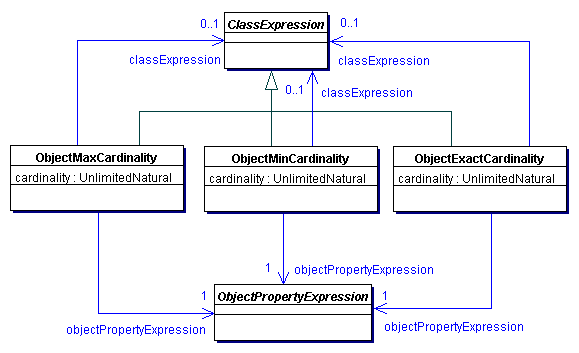
\includegraphics[width=150mm]{Figures/ce_2.png}
	\caption{Object Property Cardinality Restrictions trong OWL 2\label{overflow}}
\end{figure}
Các mô tả lớp trong OWL 2 có thể được tạo ra bằng cách đặt ra những số lượng hạn chế các cá thể mà các thuộc tính đối tượng có thể liên kết.
\subparagraph{Số lượng tối thiểu (Minimum Cardinality)} - mô tả \textit{ObjectMinCardinality(n OPE  CE)} biểu diễn mọi các thể được kết nối bởi mô tả thuộc tính đối tượng \textit{OPE} đến số lượng tối thiểu $n$ cá thể (khác nhau) thuộc mô tả lớp \textit{CE} với $n$ là số nguyên không âm. Nếu \textit{CE} không được khai báo trong phát biểu trên mặc định sẽ là $owl:Thing$. Ví dụ:
\begin{verbatim}
ObjectPropertyAssertion( a:fatherOf a:Peter a:Steve )
ObjectPropertyAssertion( a:fatherOf a:Peter a:Bush )
ClassAssertion( a:Kid a:Steve )
ClassAssertion( a:Kid a:Bush )
\end{verbatim}
\textbf{Giải thích:} với các điều kiện như trên thì Peter sẽ được ngầm hiểu thành viên của mô tả lớp sau 
$ObjectMinCardinality($ 2 a:fatherOf a:Kid $)$ - Peter là bố của ít nhất 2 đứa trẻ.

\subparagraph{Số lượng tối đa (Maximum Cardinality)} Mô tả \textit{ObjectMaxCardinality( n OPE CE)} biểu diễn mọi các thể được kết nối bởi mô tả thuộc tính đối tượng $OPE$ đến số lượng tối đa $n$ cá thể (khác nhau) thuộc mô tả lớp \textit{CE} với $n$ là số nguyên không âm. Nếu $CE$ không được khai báo trong phát biểu trên mặc định sẽ là \textit{owl:Thing}. Ví dụ:
\begin{verbatim}
ObjectPropertyAssertion( a:hasPet a:Peter a:Tom)
// Peter có vật nuôi là Tom
ClassAssertion( ObjectMaxCardinality( 1 a:hasPet ) a:Peter )
// Peter thuộc lớp "những ai có tối đa 1 vật nuôi"
\end{verbatim}
\textbf{Giải thích:} theo 2 điều kiệu trên thì Peter sẽ thuộc mô tả lớp \textit{ObjectMaxCardinality( 2 a:hasPet )} chỉ những "ai có tối đa 2 vật nuôi" (số vật nuôi <= 2), vì 2 phát biểu đầu tiên chỉ ra rằng Peter chắc chắn chỉ có một vật nuôi.

\subparagraph{Số lượng chính xác (Exact Cardinality)} - mô tả \textit{ObjectExactCardinality( n OPE CE)} biểu diễn mọi các thể được kết nối bởi mô tả thuộc tính đối tượng \textit{OPE} đến số lượng chính xác $n$ cá thể (khác nhau) thuộc mô tả lớp $CE$ với $n$ là số nguyên không âm. Nếu \textit{CE} không được khai báo trong phát biểu trên mặc định sẽ là \textit{owl:Thing}. Mô tả lớp này tương được khi lấy giao của 2 mô tả số lượng tối đa và số lượng tối thiểu cùng $n$.
\begin{verbatim}
ObjectIntersectionOf( ObjectMinCardinality( n OPE CE ) 
ObjectMaxCardinality( n OPE CE ) ).
\end{verbatim}

% Data Property Restrictions
\paragraph{Ràng buộc theo thuộc tính dữ liệu (Data Property Restrictions)}
\begin{figure}[h]
	\centering
	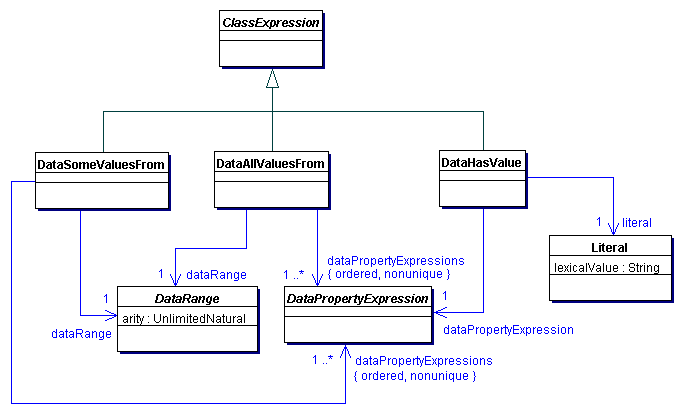
\includegraphics[width=150mm]{Figures/ce_3.png}
	\caption{Data Property Restrictions trong OWL 2\label{overflow}}
\end{figure}
Mô tả lớp dạng này được tạo ra bằng cách đặc các ràng buộc về kiểu dữ liệu, giới hạn các giá trị dữ liệu lên mô tả thuộc tính dữ liệu (data property expression) như trong hình. Những mô tả này cũng tương tự như ràng buộc thuộc tính đối tượng vừa nêu ra ở trên.

%% Existential Quantification
\subparagraph{Existential Quantification} Một mô tả lớp \textit{DataSomeValuesFrom(} $DPE_{1}$ ... $DPE_{n}$ $DR$ \textit{)} gồm $n$ mô tả thuộc tính dữ liệu $DPE_{i}$, $1<=i<=n$, và một miền dữ liệu (data range) $DR$ với số lượng tham số phải bằng $n$. Mô tả lớp này biểu diễn mối quan hệ dữ liệu giữa tất cả các cá thể kết nối với $DPE_{i}$ tới các trực nghĩa $lt_{i}$, $1<=i<=n$ với $($ $lt_{1}$ ... $lt_{n}$ $)$ trong $DR$. Ví dụ:
\begin{verbatim}
DataPropertyAssertion( a:hasAge a:Steve "17"^^xsd:integer ) // Steve 17 tuổi.
\end{verbatim}
\textbf{Giải thích:} Vì Steve 17 tuổi nên chúng ta ngầm hiểu rằng Steve thuộc những ai có số tuổi là số nguyên và không lớn hơn 20 tuổi, tương đương phát biểu sau
\begin{verbatim}
DataSomeValuesFrom( a:hasAge 
DatatypeRestriction( xsd:integer xsd:maxExclusive "20"^^xsd:integer ) )
\end{verbatim}

%% Universal Quantification
\subparagraph{Universal Quantification} Một mô tả lớp \textit{DataAllValuesFrom(} $DPE_{1}$ ... $DPE_{n}$ $DR$ \textit{)} gồm $n$ mô tả thuộc tính dữ liệu $DPE_{i}$, $1<=i<=n$, và một miền dữ liệu (data range) $DR$ với số lượng tham số phải bằng $n$. Mô tả lớp này biểu diễn mối quan hệ dữ liệu giữa tất cả các cá thể \textbf{chỉ} \textit{(only)} kết nối với $DPE_{i}$ tới các trực nghĩa $lt_{i}$, $1<=i<=n$ với $($ $lt_{1}$ ... $lt_{n}$ $)$ trong $DR$. Ví dụ: 
\begin{verbatim}
DataPropertyAssertion( a:hasZIP _:a1 "70000"^^xsd:integer ) 
// Mã vùng của _:a1 là số nguyên 70000
FunctionalDataProperty( a:hasZIP) 
// Mỗi đối tượng chỉ có duy nhất một mã vùng
\end{verbatim}
\textbf{Giải thích:} Mã vùng của một số quốc gia như Anh và Canada là dạng chuỗi (chứa ký tự và số), dựa vào 2 phát biểu trên chúng ta có thể hiểu rằng mã vùng của \verb|_a:1| thuộc mô tả những mã vùng \textbf{chỉ} gồm số nguyên $DataAllValuesFrom( a:hasZIP xsd:integer )$

% Literal Value Restriction
\subparagraph{Ràng buộc bằng giá trị trực nghĩa - Literal Value Restriction}
Một mô tả \textit{DataHasValue(} $DPE$ $lt$ \textit{)} gồm một mô tả thuộc tính dữ liệu \textit{DPE} và một trực nghĩa $lt$, nó biểu diễn quan hệ của những cá thể nào qua \textit{DPE} tới $lt$. Ví dụ:
\begin{verbatim}
DataPropertyAssertion( a:hasAge a:Steve "17"^^xsd:integer )
\end{verbatim}
\textbf{Giải thích:} Steve là thành viên của mô tả lớp sau mà không cần khai báo "những ai 17 tuổi".
\begin{verbatim}
DataHasValue( a:hasAge "17"^^xsd:integer )
\end{verbatim}

% Data Property Cardinality Restrictions
\paragraph{Ràng buộc thuộc tính dữ liệu theo số lượng}
\begin{figure}[h]
	\centering
	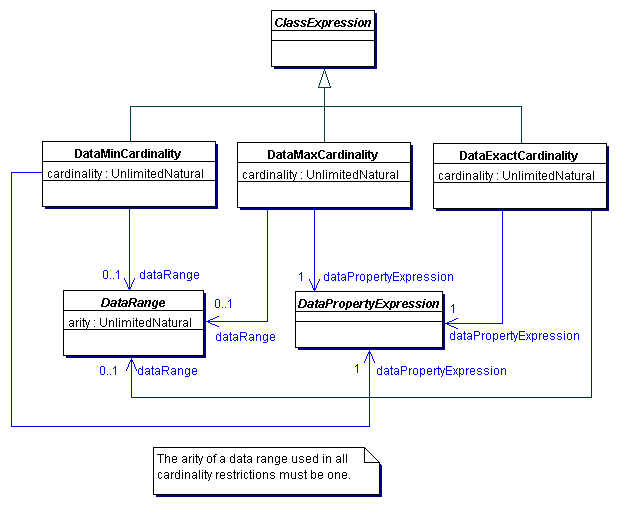
\includegraphics[width=150mm]{Figures/ce_4.png}
	\caption{Data Property Cardinality Restrictions trong OWL 2\label{overflow}}
\end{figure}
Tương tự ràng buộc thuộc tính đối tượng theo số lượng, OWL 2 cũng cho phép chúng ta tạo ra các mô tả lớp bằng cách các giá trị dữ liệu ( thay vì cá thể) mà thuộc tính dữ liệu có thể liên kết đến. Cấu trúc được mô tả như trong hình.

%% Minimum Cardinality)
\subparagraph{Số lượng tối thiểu (Minimum Cardinality)} Một mô tả lớp \textit{DataMinCardinality( n DPE DR)}  biểu diễn mọi cá thể được kết nối bởi thuộc tính dữ liệu \textit{DPE} đến số lượng tối thiểu $n$ các trực nghĩa khác nhau thuộc miền dữ liệu  \textit{DR} với $n$ số nguyên không âm. Nếu \textit{DR} không được khai báo trong phát biểu trên mặc định sẽ là \textit{rdfs:Literal}. Ví dụ:
\begin{verbatim}
DataPropertyAssertion( a:hasPhoneNumber a:Steve "0123456789" )
DataPropertyAssertion( a:hasPhoneNumber a:Steve "0987654321" )
\end{verbatim}
\textbf{Giải thích:} Với 2 phát biểu như trên tồn tại, có thể hiểu Steve thuộc lớp những ai có ít nhất 2 số điện thoại \textit{DataMinCardinality(2 a:hasPhoneNumber)}.

%% Maximum Cardinality
\subparagraph{Số lượng tối đa (Maximum Cardinality)} Một mô tả lớp \textit{DataMaxCardinality( n DPE DR)} biểu diễn mọi cá thể được kết nối bởi thuộc tính dữ liệu $DPE$ đến số lượng tối đa $n$ các trực nghĩa khác nhau thuộc miền dữ liệu  $DR$ với $n$ số nguyên không âm. Nếu $DR$ không được khai báo trong phát biểu trên mặc định sẽ là $rdfs:Literal$. Ví dụ:
\begin{verbatim}
DataPropertyAssertion( a:hasID a:Steve "0001" ) // Steve số CMND là 0001
FunctionalDataProperty( a:hasID ) // Mỗi người chỉ có duy nhất một số CMND
\end{verbatim}
\textbf{Giải thích:} Với 2 phát biểu như trên tồn tại, có thể hiểu Steve thuộc lớp "những ai có nhiều nhất 2 số CMND" ( số CMND <=2), \textit{DataMaxCardinality(2 a:hasID)}.

%% Exact Cardinality
\subparagraph{Số lượng chính xác (Exact Cardinality)} Một mô tả lớp \textit{DataExactCardinality( n DPE DR)}  biểu diễn mọi cá thể được kết nối bởi thuộc tính dữ liệu \textit{DPE} đến số lượng chính xác $n$ các trực nghĩa khác nhau thuộc miền dữ liệu  \textit{DR} với $n$ số nguyên không âm. Nếu \textit{DR} không được khai báo trong phát biểu trên mặc định sẽ là \textit{rdfs:Literal}. Ví dụ:
\begin{verbatim}
DataPropertyAssertion( a:hasID a:Steve "0001" ) // Steve số CMND là 0001
FunctionalDataProperty( a:hasID ) // Mỗi người chỉ có duy nhất một số CMND
\end{verbatim}
\textbf{Giải thích:} Với 2 phát biểu như trên tồn tại, có thể hiểu Steve thuộc lớp "có duy nhất 1 CMND" \textit{DataExactCardinality(1 a:hasName)}.

% Axioms
\subsubsection{Các tiên đề (Axioms)}
{\let\thefootnote\relax\footnotetext{* Lưu ý:\textit{
			Trong nội dung báo cáo này chúng em sẽ gọi vắng tắt các tiên đề - những phát biểu hiển nhiên đúng trong một lĩnh vực là \textit{những phát biểu} nhằm diễn giải các lý thuyết, nguyên lý trở dễ hiểu hơn.
		}}
	}
	Thành phần chính của một OWL 2 Ontology chính là một tập hợp gồm các tiên đề \textsuperscript{*} - những phát biểu mà chúng ta cho là đúng trong một lĩnh vực. OWL 2 cung cấp một loạt các loại phát biểu được mở rộng (thừa kế) từ lớp \textbf{Axiom} như trong hình. Các phát biểu có thể là các phát biểu khai báo (declarations), phát biểu về lớp, phát biểu về thuộc tính đối tượng/dữ liệu, phát biểu định nghĩa kiểu dữ liệu, khóa (HasKey), phát biểu khẳng định (assertions), và các phát biểu chú thích (annotations). Có thể nói những phát biểu (tiên đề) chính là những viên gạch để chúng ta xây dựng nên các tầng ngữ nghĩa (semantic) cho ontology.
	\begin{figure}[!h]
		\centering
		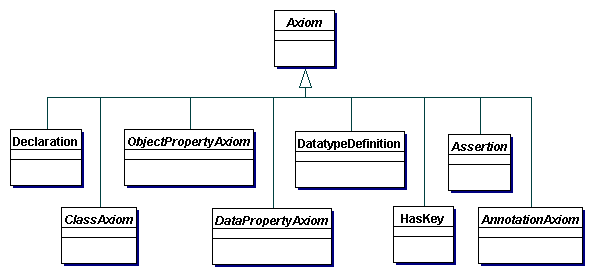
\includegraphics[width=150mm]{Figures/axioms.png}
		\caption{Các dạng phát biểu của OWL 2\label{overflow}}
	\end{figure}
	
	\paragraph{Những phát biểu về mô tả lớp - Class Expression Axioms}
	Những phát biểu này cho phép biểu diễn các loại quan hệ giữa những mô tả lớp (Class Expressions) với nhau. Có 4 phát biểu được mở rộng ra từ phát biểu này như trong hình.
	\begin{figure}[!h]
		\centering
		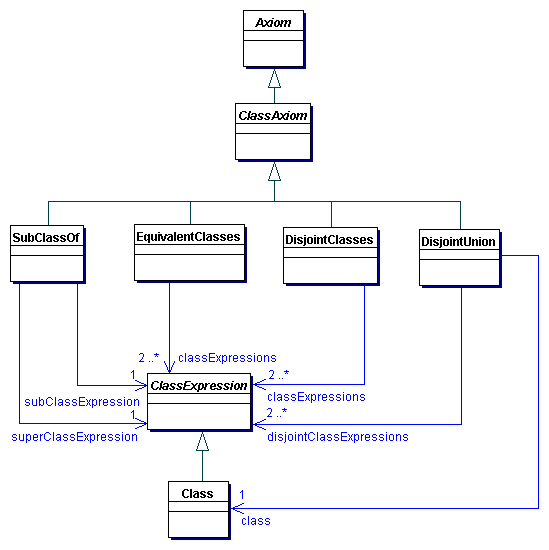
\includegraphics[width=120mm]{Figures/classAxiom.png}
		\caption{Các dạng phát biểu về lớp của OWL 2\label{overflow}}
	\end{figure}
	
	\subparagraph{Phát biểu lớp con (SubClass Axioms)} - một phát biểu \textit{SubClassOf(}$CE_{1}$ $CE_{2}$ \textit{)} nói rằng mô tả lớp $CE_{1}$ là lớp con của mô tả lớp $CE_{2}$. Phát biểu này là phát biểu cơ bản trong OWL 2 được sử dụng để xây dựng một phân cấp lớp trong Ontology. Ví dụ:
	\begin{verbatim}
	SubClassOf( a:Driver a:Adult ) // Mỗi tài xế là một người trưởng thành.
	SubClassOf( a:Adult a:Person ) // Mỗi người trưởng thành là một người.
	ClassAssertion (a:Driver a:Steve ) // Steve là một tài xế.
	\end{verbatim}
	\textbf{Giải thích:} nhờ 2 phát biểu đầu tiên, chúng ta ngầm hiểu tài xế cũng là một người trưởng thành, cũng là một người, vì vậy tất cả những cá thể là tài xế, cũng là người trưởng thành và cũng là người -> Steve là cũng là thành viên của 2 lớp $Adult$ và $Person$.
	
	\subparagraph{Phát biểu lớp tương đương (Equivalent Classes)} - một phát biểu \textit{EquivalentClasses( $CE_{1}$ $CE_{n}$ )} nói rằng mỗi mô tả lớp $CE_{i}$, $1<=i<=n$ đều đồng nghĩa với các tất cả các mô tả lớp còn lại trong phát biểu này. Phát biểu \textit{EquivalentClasses( $CE_{2}$ $CE_{1}$ )} tương đương \textit{EquivalentClasses( $CE_{1}$ $CE_{2}$ )}. Ví dụ:
	\begin{verbatim}
	SubClassOf( a:Bike  a:Bicycle )
	\end{verbatim}
	
	\subparagraph{Disjoint Classes} - một phát biểu \textit{DisjointClasses( $CE_{1}$ ... $CE_{n}$ )}nói rằng không cá thể nào của $CE_{i}$ thuộc $CE_{j}$ và ngược lại với $i \neq j$, $1<=i,j<=n$. Ví dụ:
	\begin{verbatim}
	DisjointClasses( a:Man a:Woman )	
	ClassAssertion( a:Man a:Steve )
	\end{verbatim}
	\textbf{Giải thích:} Steve không là nữ - \textit{ObjectComplementOf( a:Girl )}, nếu chúng ta khai báo thêm $ClassAssertion($ $a:Girl$ $a:Steve)$ sẽ làm cho ontology bị thiếu tính nhất quán (sẽ được nếu rõ hơn ở các chương sau).
	
	\paragraph{Phát biểu về thuộc tính đối tượng (Object Property Axioms)}
	Những phát biểu này cho phép biểu diễn các loại quan hệ giữa những mô tả thuộc tính đối tượng (Object Property Expressions) với nhau.
	\begin{figure}[h]
		\centering
		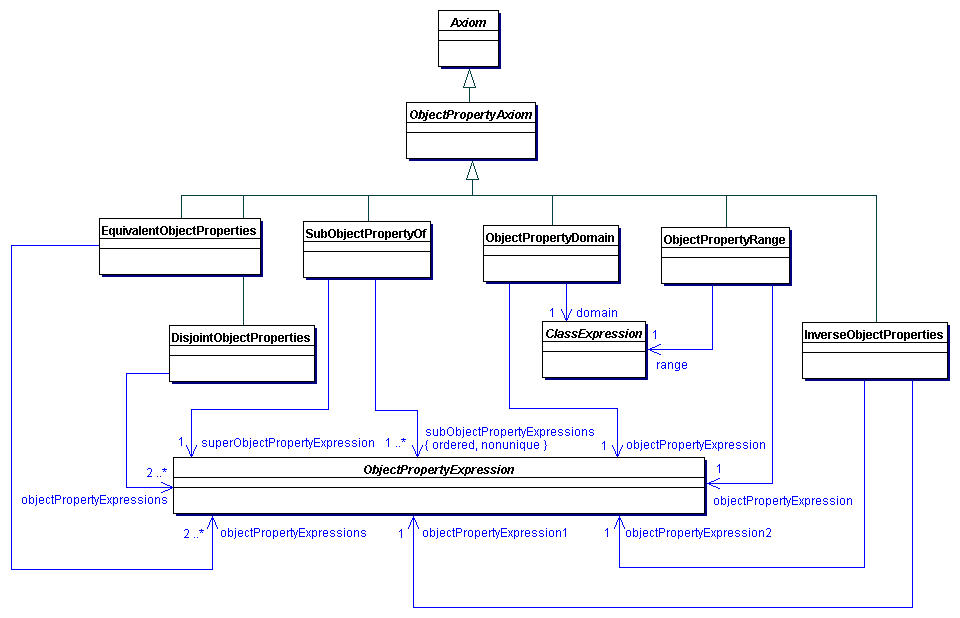
\includegraphics[width=160mm]{Figures/objectpropertyAxiom.png}
		\caption{Các dạng phát biểu về thuộc tính đối tượng của OWL 2 (phần 1)\label{overflow}}
	\end{figure}
	
	\subparagraph{Thuộc tính đối tượng con (SubObjectPropertyOf)} - một phát biểu \textit{SubObjectPropertyOf( $OPE_{1}$ $OPE_{2}$ )} nói rằng mô tả thuộc tính đối tượng $OPE_{1}$ là thuộc tính con của mô tả thuộc tính đối tượng $OPE_{2}$, có nghĩa nếu một cá thể $x$ được liên kết bởi $OPE_{1}$ với $y$ thì $x$ cũng được liên kết bởi $OPE_{2}$ đến $y$. Ví dụ:
	\begin{verbatim}
	SubObjectPropertyOf( a:hasCat a:hasPet )     
	ObjectPropertyAssertion( a:hasCat a:Peter a:Tom) // Peter có con mèo là Tom
	\end{verbatim}
	\textbf{Giải thích:} Ai có mèo thì cũng có thể hiểu là người đó có vật nuôi theo phát biểu đầu tiên, dựa theo phát biểu thứ hai chúng ta có ngầm hiểu là \textit{Peter có vật nuôi là Tom} - \textit{ObjectPropertyAssertion( a:hasPet a:Peter a:Brian )}.
	
	\subparagraph{Thuộc tính đối tượng tương đương (Equivalent Object Properties)} - một phát biểu \textit{EquivalentObjectProperties( $OPE_{1}$ ... $OPE_{n}$ )} nói rằng mỗi mô tả thuộc tính $OPE_{i}$, $1<=i<=n$ đều đồng nghĩa với các tất cả các mô tả thuộc tính còn lại trong phát biểu này phát biểu \textit{EquivalentObjectProperties( $OPE_{2}$ $OPE_{1}$ )} tương đương \textit{EquivalentObjectProperties( $OPE_{1}$ $OPE_{2}$ )}. Ví dụ:
	\begin{verbatim}
	EquivalentObjectProperties( a:hasBrother a:hasMaleSibling ) 
	ObjectPropertyAssertion( a:hasBrother a:Chris a:Steve )     
	// Steve là anh của Chris
	ObjectPropertyAssertion( a:hasMaleSibling a:Steve a:Chris ) 
	// Chris là anh chị em ruột (mà là nam) của Steve
	\end{verbatim}
	\textbf{Giải thích:} Do phát biểu đầu tiên có nghĩa "có anh" đồng nghĩa với "có anh chị em ruột (là nam)", từ 2 phát biểu sau chúng ta có thể suy ra các phát biểu sau mà cần khai báo chúng \textit{ObjectPropertyAssertion(a:hasMaleSibling a:Chris a:Steve)} và \textit{ObjectPropertyAssertion(a:hasBrother a:Stewie a:Chris)}.
	
	\subparagraph{Disjoint Object Properties} - một phát biểu \textit{DisjointObjectProperties($OPE_{1}$ ... $OPE_{n}$)} nói rằng không cá thể được liên kết bởi cả của $OPE_{i}$ và $OPE_{j}$ với $i \neq j$, $1<=i,j<=n$. Ví dụ:
	\begin{verbatim}
	DisjointObjectProperties( a:hasFather a:hasMother ) Có ba khác có mẹ.
	ObjectPropertyAssertion( a:hasFather a:Steve a:Peter )	Peter là ba của Steve.
	ObjectPropertyAssertion( a:hasMother a:Steve a:Lois ) Lois là mẹ của Steve.
	\end{verbatim}
	Nếu thêm phát biểu \textit{ObjectPropertyAssertion(a:hasMother a:Steve a:Peter)} sẽ dẫn đến tính thiếu nhất quán.
	
	\subparagraph{Thuộc tính đối tượng nghịch đảo} - \textit{phát biểu InverseObjectProperties( $OPE_{1}$ $OPE_{2}$ )} nói rằng thuộc tính đối tượng $OPE_{2}$ là nghịch đảo của $OPE_{1}$. Nếu cá thể $x$ được kết nối bởi $OPE_{1}$ tới cá thể $y$, thì $y$ sẽ được kết nối bởi $OPE_{2}$ tới $x$ và ngược lại. Ví dụ:
	\begin{verbatim}
	InverseObjectProperties( a:parentOf a:childOf )
	ObjectPropertyAssertion( a:childOf a:Peter a:Steve ) 
	// Steve là con của Peter
	\end{verbatim}
	\textbf{Giải thích:} Phát biểu đầu có thể hiểu "nếu x là con y" thì "y là ba mẹ của x", do vậy từ các phát biểu trên ta suy ra được Peter là ba mẹ của Steve tương đương \textit{ObjectPropertyAssertion( a:parentOf a:Steve a:Peter)}.
	
	\subparagraph{Domain của thuộc tính đối tượng (Object Property Domain)} - phát biểu \textit{ObjectPropertyDomain(OPE CE)} nêu rõ domain của thuộc tính đối tượng là mô tả lớp \textit{CE} -  nếu một cá thể $x$ được liên kết bởi \textit{OPE} tới cá thể nào đó, thì $x$ phải thuộc mô tả lớp \textit{CE}. Mặc định nếu không có khai báo này thì domain thuộc tính đối tượng sẽ là \textit{owl:Thing}
	\begin{verbatim}
	ObjectProertyDomain( a:hasCat a:Person ) 
	// Con người mới nuôi mèo
	ObjectPropertyAssertion( a:hasCat a:Peter a:Tom ) 
	// Tom là con mèo của Peter
	\end{verbatim}
	\textbf{Giải thích:} Mặc dù không khai báo Peter là người nhưng xét theo phát biểu đầu tiên chúng ta ngầm hiểu Peter là người, tương đương phát biểu \textit{ClassAssertion(a:Person a:Peter)}.
	
	\subparagraph{Miền giới hạn của thuộc tính đối tượng (Object Property Range)} - phát biểu \textit{ObjectPropertyRange( $OPE$ $CE$)} nêu rõ miền giới hạn (range) của thuộc tính đối tượng là mô tả lớp \textit{CE} -  nếu cá thể nào đó được liên kết bới $OPE$ tới cá thể $x$ , thì $x$ phải thuộc mô tả lớp $CE$. Mặc định nếu không có khai báo này thì range của thuộc tính đối tượng sẽ là $owl:Thing$. Ví dụ:
	\begin{verbatim}
	ObjectProertyRange( a:hasPet a:Cat ) 
	// ai có vật nuôi thì bắt buộc đó phải là con mèo
	ObjectPropertyAssertion( a:hasPet a:Peter a:Tom ) 
	// Tom là vật nuôi của Peter
	\end{verbatim}
	\textbf{Giải thích:} Mặc dù không khai báo Tom là con mèo nhưng do phát biểu đầu tiên, chúng ta ngầm hiều Tom là con mèo, tương đương phát biểu \textit{ClassAssertion($a:Cat$ $a:Tom$)}.
	
	\begin{figure}[h]
		\centering
		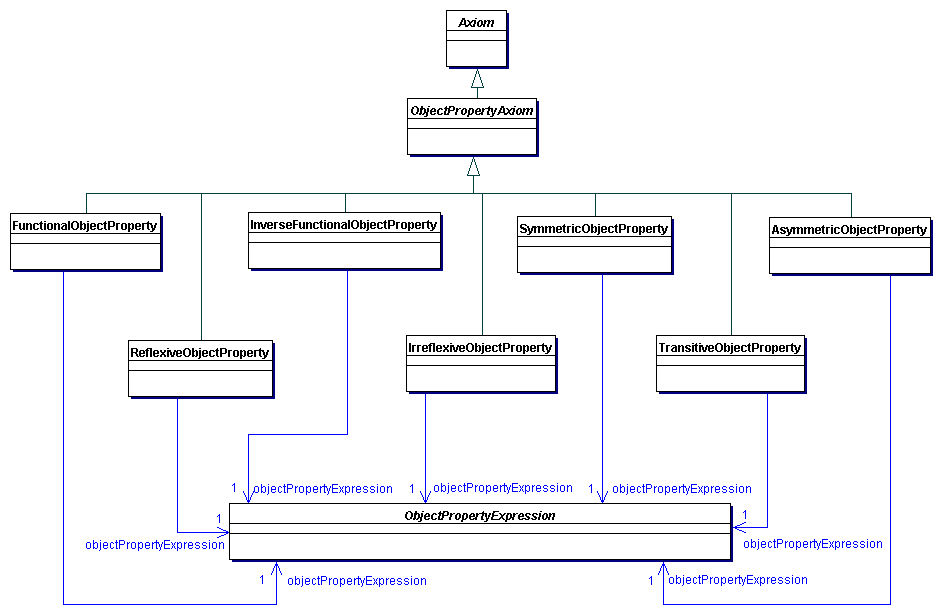
\includegraphics[width=150mm, height=100mm]{Figures/objectpropertyAxiom1.png}
		\caption{Các dạng phát biểu về thuộc tính đối tượng của OWL 2 (phần 2) \label{overflow}}
	\end{figure}
	Ngoài các dạng phát biểu được nêu, mô tả thuộc tính đối tượng còn có thêm các phát biểu trong hình sau, nhằm quy định tính chất của mô tả thuộc tính đối tượng hay giữa các cá thể được kết nối bằng các thuộc tính đối tượng này, chẳng hạn thuộc tính\textit{ SymmetricObjectProperty} quy định mô tả thuộc tính đối tượng có tính đối xứng - nếu $x$ là bạn $y$ thì $y$ cũng là bạn $x$. 
	
	\subparagraph{Functional Object Properties} phát biểu \textit{FunctionalObjectProperty( OPE )} quy định với từng cá thể $x$, chỉ tồn tại nhiều nhất một cá thể $y$ mà $x$ được kết nối với $y$ qua $OPE$. Ví dụ : Mỗi đối tượng chỉ có tối đa một người cha - \textit{FunctionalObjectProperty( a:hasFather )}. 
	
	\subparagraph{Inverse-Functional Object Properties} phát biểu \textit{InverseFunctionalObjectProperty( OPE )} quy định với từng cá thể $x$, chỉ tồn tại nhiều nhất một cá thể $y$ mà $y$ được kết nối qua \textit{OPE} tới $x$ . Ví dụ tương tự \textit{FunctionalObjectProperty(OPE)}.
	
	\subparagraph{Reflexive Object Properties} phát biểu \textit{ReflexiveObjectProperty( OPE )} nói rằng mô tả thuộc tính có tính phản xạ, nghĩa là với từng kết nối bởi \textit{OPE} tới chính nó. Ví dụ: \textit{ReflexiveObjectProperty(a:knows)}, ai cũng biết bản thân họ, với khai báo \textit{ClassAssertion(a:Person a:Peter)} thì có thể suy ra được phát biểu sau \textit{ObjectPropertyAssertion(a:knows a:Peter a:Peter)}.
	
	\subparagraph{Irreflexive Object Properties} ngược lại với phát biểu trên  \textit{IrreflexiveObjectProperty( OPE )}, không có cá thể nào tự kết nối với chính nó qua \textit{OPE}. Ví dụ: \textit{IrreflexiveObjectProperty(a:marriedTo)}, không ai cưới chính mình.
	
	\subparagraph{Symmetric Object Properties} phát biểu \textit{SymmetricObjectProperty( OPE )} nói rằng \textit{OPE} có tính đối xứng, nếu $x$ nối với $y$ qua \textit{OPE} thì $y$ cũng nối với $x$ bởi \textit{OPE}. Ví dụ: Với\textit{ SymmetricObjectProperty( a:friendOf )} và \textit{ObjectPropertyAssertion(a:friend a:Peter a:Bush)} chúng ta suy ra được \textit{ObjectPropertyAssertion(a:friend a:Bush a:Peter)}.
	
	\subparagraph{Asymmetric Object Properties} phát biểu \textit{AsymmetricObjectProperty( OPE )} nói rằng \textit{OPE} có tính bất đối xứng, nếu $x$ nối với $y$ qua \textit{OPE}, thì $y$ không thể kết nối với $x$ bởi \textit{OPE}. Ví dụ: Với \textit{AsymmetricObjectProperty( a:parentOf )}  và \textit{ObjectPropertyAssertion(a:parentOf a:Peter a:Bush)} thì nếu ta thêm thêm phát biểu \textit{ObjectPropertyAssertion(a:parentOf a:Bush a:Peter)} sẽ làm cho ontology mất tính nhất quán (inconsistent).
	
	\subparagraph{Transitive Object Properties} phát biểu \textit{TransitiveObjectProperty(OPE)} nói rằng \textit{OPE} có tính bắc cầu, nếu $x$ nối với $y$ bởi \textit{OPE} và $y$ nối với $z$ cũng bằng \textit{OPE} thì $x$ nối với $z$ qua \textit{OPE}. Ví dụ:
	\begin{verbatim}
	TransitiveObjectProperty( a:partOf ) 
	ObjectPropertyAssertion( a:partOf a:KhoaMMT a:UIT )
	ObjectPropertyAssertion( a:partOf a:UIT a:VNU )
	\end{verbatim}
	Giải thích nếu khoa mạng thuộc UIT, UIT thuộc đại học Quốc Gia (VNU), nhờ phát biểu đầu tiên chúng ta $partOf$ có tính chất bắc cầu nên suy ra được khoa mạng thuộc đại học Quốc Gia - \textit{ObjectPropertyAssertion( a:partOf a:KhoaMMT a:VNU)}
	
	% Data Property Axioms
	\paragraph{Các phát biểu về thuộc tính dữ liệu}
	\begin{figure}[h]
		\centering
		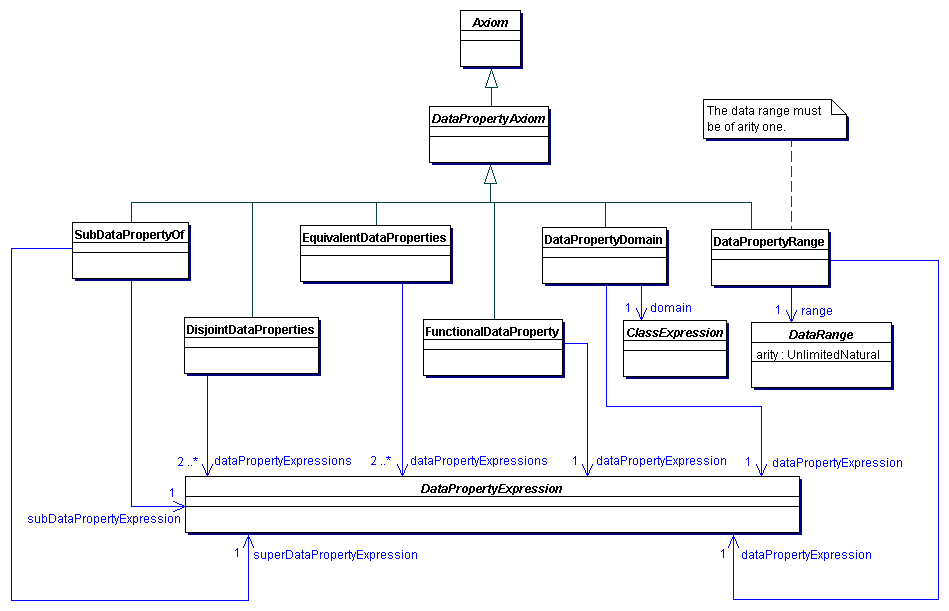
\includegraphics[width=150mm]{Figures/datapropertyAxiom.png}
		\caption{Các dạng phát biểu về thuộc tính dữ liệu của OWL 2 (phần 2) \label{overflow}}
	\end{figure}
	Cũng giống như mô tả thuộc tính đối tượng, mô tả thuộc tính dữ liệu cũng được cung cấp các phát biểu như \textit{SubDataPropertyOf}, \textit{EquivalentDataProperties}, \textit{DataPropertyDomain}, \textit{DataProperyRange}.
	
	\subparagraph{Phát biểu thuộc tính dữ liệu con (Data subproperties)} Phát biểu SubDataPropertyOf( $DPE_{1}$ $DPE_{2}$ ) nói rằng mô tả thuộc tính dữ liệu $DPE_{1}$ là thuộc tính con của mô tả dữ liệu $DPE_{2}$ - có nghĩa nếu một cá thể $x$ được kết nối bởi $DPE_{1}$ tới một trực nghĩa $y$, thì $x$ được kết nối bởi $DPE_{2}$. Ví dụ:
	\begin{verbatim}
	SubDataPropertyOf( a:hasLastName a:hasName) 
	// Họ của một người cũng là tên họ của người đó
	DataPropertyAssertion( a:hasLastName a:Peter "Smith" )
	// Họ của Peter là "Smith"
	\end{verbatim}
	\textbf{Giải thích:} Vì "có họ" \textbf{(hasLastName)} là thuộc tính con của "có tên" \textit{(hasName)} nên chúng ta ngầm hiểu phát biểu sau mà không cần khai báo tên của Peter là "Smith", tương đương \textit{DataPropertyAssertion(a:hasName a:Peter "Griffin")}
	
	\subparagraph{Phát biểu thuộc tính dữ liệu tương đương (Equivalent Data Properties)} Một phát biểu \textit{EquivalentDataProperties( $DPE_{1}$ ... $DPE_{n}$)} nói rằng mỗi mô tả thuộc tính $DPE_{i}$, $1<=i<=n$ đều đồng nghĩa với các tất cả các mô tả thuộc tính còn lại trong phát biểu này phát biểu \textit{EquivalentDataProperties( $DPE_{2}$ $DPE_{1}$ )} cũng tương đương EquivalentDataProperties( $DPE_{1}$ $DPE_{2}$ ). Ví dụ:
	\begin{verbatim}
	EquivalentDataProperties( a:hasName a:HoTen ) 
	// a:hasName tương đượng với a:HoTen trong Tiếng Việt
	DataPropertyAssertion( a:hasName a:Peter "Peter Nguyen" )
	DataPropertyAssertion( a:HoTen a:Peter "Peter Nguyễn" )
	\end{verbatim}
	\textbf{Giải thích:} Do phát biểu đầu tiên, từ phát biểu thứ 2 ta ngầm hiểu \textit{DataPropertyAssertion( a:hasName a:Peter "Peter Nguyễn" )} tên tiếng Anh "Peter Nguyen" tương đương tên tiếng Viết "Peter Nguyễn" và ngược lại \textit{DataPropertyAssertion( a:HoTen $a:Peter$ "Peter Nguyen") }.
	
	\subparagraph{Domain của thuộc tính dữ liệu (Data Property Domain)} Phát biểu \textit{DataPropertyDomain( DPE CE )} nêu rõ domain của thuộc tính dữ liệu là mô tả lớp $CE$ -  nếu một cá thể $x$ được liên kết bởi \textit{DPE} tới vài trực nghĩa nào đó, thì $x$ phải là cá thể thuộc mô tả lớp \textit{CE}.
	\begin{verbatim}
	DataPropertyDomain( a:hasBankAccount a:Person ) 
	// Con người mới có tài khoản ngân hàng
	ObjectPropertyAssertion( a:hasBankAccount a:Peter "0002" ) 
	// Peter có tài khoản ngân hàng "0002"
	\end{verbatim}
	\textbf{Giải thích:} Không cần thiết phải khai báo Peter là người vì dựa theo chúng ta cũng kết luận được Peter là người từ 2 phát biểu trên, \textit{ClassAssertion(a:Person a:Peter)}.
	
	\subparagraph{Miền giá trị của thuộc tính dữ liệu (Data Property Range)} - phát biểu \textit{DataPropertyRange(DPE DR)} nói rằng miền giá trị hợp lệ của mô tả thuộc tính dữ liệu \textit{DPE} là miền dữ liệu \textit{DR} - nếu các cá thể được kết nối bởi \textit{DPE} tới 1 trực nghĩa $x$, thì $x$ trong miền dữ liệu \textit{DR}. Ví dụ:
	%Số lượng kết quả đầu ra bắt buộc bằng 1, tức không tồn tại $x \equiv y \equiv z$, với $y \not\equiv z$ và $y, z \in DR$.
	\begin{verbatim}
	DataPropertyRange( a:hasName xsd:string )
	DataPropertyAssertion( a:hasName a:Peter "Peter Nguyen" )
	\end{verbatim}
	Nếu khai báo thêm phát biểu sau sẽ làm cho ontology bị thiếu nhất quán (inconsistent):
	\begin{verbatim}
	DataPropertyAssertion( a:hasName a:Peter "42"^^xsd:integer)
	\end{verbatim}
	
	\subparagraph{Functional Data Properties} - phát biểu \textit{FunctionalDataProperty(DPE)} nói rằng với mỗi $x$, chỉ có nhiều nhất một trực nghĩa $y$ mà $x$ được gán cho bởi \textit{DPE}. Ví dụ:
	\begin{verbatim}
	FunctionalDataProperty( a:hasAge )
	// Mọi đối tượng chỉ có tối đa một số tuổi
	DataPropertyAssertion( a:hasAge a:Steve "17"^^xsd:integer )
	\end{verbatim}
	Các phát biểu trên sẽ bị thiếu nhất quán nếu chúng ta thêm vào phát biểu sau :
	\begin{verbatim}
	DataPropertyAssertion( a:hasAge a:Steve "15"^^xsd:integer)
	\end{verbatim}
	
	%% Assertions
	\paragraph{Các phát biểu về cá thể (Assertions)} 
	\begin{figure}[H]
		\centering
		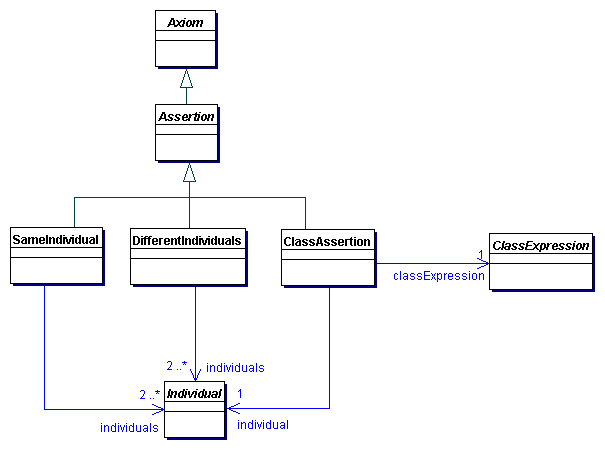
\includegraphics[width=120mm]{Figures/abox1.png}
		\caption{Các phát biểu gán lớp cho cá thể và cá thể giống nhau/khác nhau trong OWL 2 \label{overflow}}
	\end{figure}
	
	\begin{figure}[ht!]
		\centering
		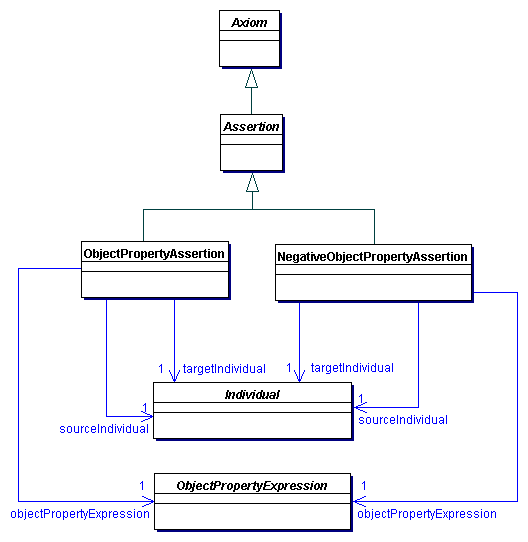
\includegraphics[width=120mm,height=110mm]{Figures/abox2.png}
		\caption{Các phát biểu về thuộc tính đối trượng của cá thể trong OWL 2 \label{overflow}}
	\end{figure}
	
	\begin{figure}[hb!]
		\centering
		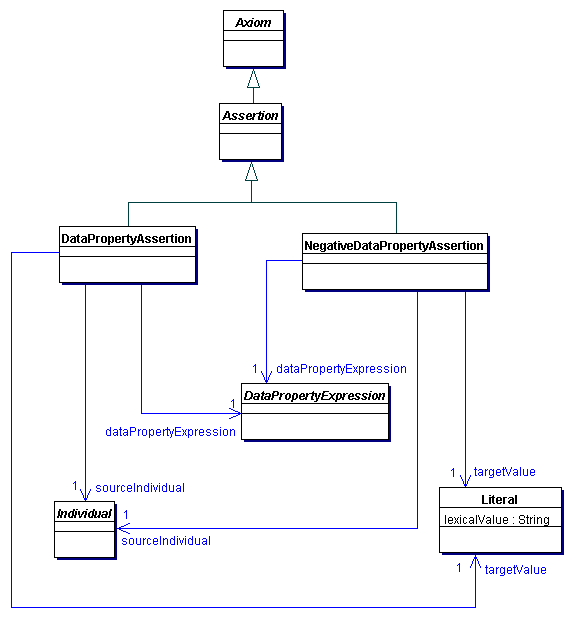
\includegraphics[width=120mm,height=110mm]{Figures/abox3.png}
		\caption{Các phát biểu về thuộc tính dữ liệu của cá thể trong OWL 2 \label{overflow}}
	\end{figure}
	Các phát biểu về cá thể thường được gọi là \textit{facts}. Để rõ hơn, các loại assertions khác nhau được thể hiện trong các hình sau.
	
	\begin{description}
		\item[SameIndividual] - khẳng định sự tương đồng của các cá thể trong phát biểu.
		
		\item[DifferentIndividuals] - khẳng định sự khác nhau của các cá thể trong phát biểu.
		
		\item[ClassAssertion] - khẳng định một cá thể thuộc một mô tả lớp/ lớp cụ thể trong phát biểu.
		
		\item[ObjectPropertyAssertion] - khẳng định mối quan hệ từ một cá thể tới một cá thể nào đó bởi một mô tả thuộc tính đối tượng.
		
		\item[NegativeObjectPropertyAssertion] - phủ định mối quan hệ từ một cá thể tới một cá thể khác bởi một mô tả thuộc tinh đối tượng.
		
		\item[DataPropertyAssertion] - khẳng định mối quan hệ từ một cá thể tới một trực nghĩa bởi một mô tả thuộc tính dữ liệu.
		
		\item[NegativeDataPropertyAssertion] - phủ định mối quan hệ từ một cá thể tới một trực nghĩa bởi một mô tả thuộc tính dữ liệu.
	\end{description}
	
\paragraph{Kết luận} Chúng em vừa trình bày qua những thành phần chính của OWL2 cũng như cách sử dụng của chúng trong quá trình suy luận (reasoning) nhằm tìm ra thông tin ẩn bên trong những phát biểu được khai báo, với mục tiếu cuối cùng là trình bày tính năng phân loại tự động. Vì độ dài khóa luận hạn chế, nên có một số thành phần của OWL 2 chưa được nêu ra ở đây như \textbf{Datatype Definitions}, \textbf{Keys}, \textbf{Annotations}, \textbf{Datatype Maps}. Thầy cô và các bạn có thể tham khảo thêm ở \cite{owl2spec}. Phần tiếp theo chúng em xin được giới thiệu về Semantic Web Rule Language, một ngôn ngữ điều luật có nhiệm vụ chính là tăng cường tính năng suy luận cho ngôn ngữ OWL 2.
%% ----------------------------------------------------------------
% Kết thúc OWL
%% ----------------------------------------------------------------
% Bắt đầu SWRL 
%% ----------------------------------------------------------------
\section{Semantic Web Rule Language}
Nếu chỉ sử dụng các thành phần của OWL 2 được trình bày ở chương trước thì vẫn chưa đủ diễn tả hết tất cả các mối quan hệ trong ontology. Semantic Web Rule Language (SWRL) là một ngôn ngữ điều luật tuân theo các quy ước Description Logic mà OWL 2 tuân thao \cite{swrlfaq}. SWRL cho phép người sử dụng khai báo các điều luật dựa trên các khái niệm của OWL như lớp, thuộc tính đối tượng, thuộc tính dữ liệu nhằm cung cấp một khả năng suy luận mạnh mẽ hơn so với chỉ dùng OWL 2. SWRL có ưu điểm là giúp tối ưu khả năng lập luận, tuy nhiên nó cũng có nhược điểm là dễ làm cho các phát biểu bị thiếu nhất quán (inconsistent).

\subsection{Cấu trúc của một SWRL Rule \cite{swrlfaq}}
Một luật SWRL chứa một phần điều kiện, hay còn gọi là rule body, và một phần kết quả, hay còn gọi là rule head. Cả phần body và head đều là giao của các positive atoms.
\begin{center}
	$atom$ \verb|^| $atom$ ... -> $atom$ \verb|^| $atom$ 
\end{center}
Có thể hiểu một SWRL Rule theo cách như sau : Khi tất cả các điều kiện nhỏ nhất (atom) trong phần điều kiện (body) đúng thì chắc chắn rằng những ý được nêu ra trong phần kết quả (head) cũng đúng. Một rule \textit{atom} có dạng:
\begin{center}
	$p($ $arg_{1}$, $arg_{2}$, ... $arg_{n}$ $)$
\end{center}
Trong đó $p$ là kí hiệu cho nội dung điều kiện (Predicate) và $arg_{i}$, $1<=i<=n$, là những khái niệm hay tham số của một \textit{Rule Atom}. Trong SWRL, nội dung điều kiện có thể là các lớp, các thuộc tính hoặc kiêu dữ liệu trong OWL 2. Tham số truyền vào có thể là cá thể, giá trị dữ liệu, hoặc biến để gán cho các khái niệm vừa nêu. Tên biến chỉ có hiệu lực trong cùng một rule, vì vậy có thể sử dụng lại tên biến cho 2 rule khác nhau.
\subsection{Các loại Rule Atom}
Sau đây, chúng em xin trình bày các loại \textit{Atom} trong SWRL Rule, đồng thời kèm theo những ví dụ cơ bản thể hiện tính năng quyết định dựa trên các điều kiện của SWRL.
\subsubsection{Class Atom}
Một \textbf{Class Atom} gồm một tên lớp hay mô tả lớp trong OWL2 Ontology và một tham số duy nhất đại diện cho cá thể của lớp đó. Ví dụ:
\begin{verbatim}
Person(?p)
Vehicle(?v)
Man(Peter)
\end{verbatim}
Tham số có thể là biến đại diện cho cá thể \verb|?p|, \verb|?v| hoặc tên của cá thể \verb|Peter|.
Một rule đơn giản để khẳng định rằng "ai làm nam đều là người":
\begin{verbatim}
Man(?x) -> Person(?x)
\end{verbatim}
\subsubsection{Individual Property Atom}
Một \textbf{Individual Property Atom} gồm một thuộc tính đối tượng (object property) và 2 tham số đại diện cho 2 cá thể trong OWL2 ontology, tham số có thể là biến hoặc tên của cá thể. Ví dụ:
\begin{verbatim}
hasBrother(?x, ?y)   // có anh em
hasSibling(Steve, ?y) // có anh/chị em 
\end{verbatim}
Trong ví dụ, \textit{hasBrother} và \textit{hasSibling} là các thuộc tính đối tượng, \verb|?x| và \verb|?y| là biến đại diện cho các cá thể, và \verb|Steve| là tên của một cá thể (named individual). Xem ví dụ sau:
\begin{verbatim}
Person(?p) ^ hasSibling(?p,?s) ^ Man(?s) -> hasBrother(?p,?s)
\end{verbatim}
\textbf{Giải thích:} Nếu một người \verb|?p| nào đó có một anh chị em \verb|?s| nào đó, và người \verb|?s| này là nam thì người \verb|?p| có anh/em trai là người \verb|?s|. Rule này cũng có thể được biểu diễn trong bằng các phát biểu về lớp, domain và range OWL2 như sau:
\begin{verbatim}
SubClassOf(a:Man a:Person)
SubClassOf(a:Woman a:Person)
DisjointClasses(a:Woman a:Man)
SubObjectProperty(a:hasBrother a:hasSibling)
ObjectPropertyRange(a:hasBrother a:Man)
ObjectPropertyRange(a:hasSibling a:Person)
ObjectPropertyDomain(a:hasSibling a:Person)
ObjectPropertyDomain(a:hasBrother a:Person)
\end{verbatim}
Trong trường hợp chúng ta có các khẳng định sau về 2 cá thể \verb|Peter| và \verb|Nguyen|
\begin{verbatim}
ClassAssertion(a:Person a:Peter)
ClassAssertion(a:Man a:Nguyen)
ObjectPropertyAssertion(a:hasSibling a:Peter a:Nguyen)
\end{verbatim}
Dựa vào rule đã khai báo ở trên \textit{hoặc} các phát biểu về lớp, domain, range như trên, thì các khẳng định vừa nêu sẽ suy ra cùng một kết quả đó là "Peter có anh/em trai là Nguyen" tương đương với phát biểu \textit{ObjectProperyAssertion(a:hasBrother a:Peter a:Nguyen)}.
\textbf{Nhận xét:} Qua các ví dụ này, có thể thấy rõ ràng SWRL có lợi thế hơn trong việc suy ra các ẩn ý so với việc chỉ sử dụng các phát biểu của OWL2, tuy nhiên có một nhược điểm đó là tính nhất quán (consistency) của ontology dễ bị vi phạm hơn do rule có thể xung đột với các phát biểu của OWL2. Lấy lại các phát biểu và rule trong ví dụ trên:
\begin{verbatim}
Person(?p) ^ hasSibling(?p,?s) ^ Woman(?s) -> hasBrother(?p,?s)
Person(?p) ^ hasSibling(?p,?s) ^ Man(?s) -> hasBrother(?p,?s)
ObjectPropertyRange(a:hasBrother a:Man) // Có anh/em trai
\end{verbatim}
\textbf{Giải thích:} 2 Rule mâu thuẫn với nhau do phát biểu "có anh/em trai". Bản thân SWRL sẽ không kiểm tra các mâu thuẫn này cho đến khi chúng xảy ra và làm cho ontology bị thiếu nhất quán. Vì vậy, người phát triển ontology cần cẩn thận trong việc kết hợp cả SWRL và OWL2.

\subsubsection{Data Valued Property Atom}
Một Data Valued Property Atom gồm một thuộc tính dữ liệu trong OWL2 và 2 tham số. Tham số đầu tiên được gán cho một các thể trong OWL 2, có thể là biến số hay tên của cá thể. Tham số thứ hai gán cho một giá trị dữ liệu, có thể là biến số hay giá trị. Ví dụ:
\begin{verbatim}
hasAge(?x, ?age)
hasAge(?x, 100)
hasName(?x, "Nguyen")
hasNumberOfChilds(Peter, ?x)
\end{verbatim}
Một rule đơn giản với ý nghĩa "những ai có xe, có bằng lái thì là tài xế":
\begin{verbatim}
Person(?p) ^ hasCar(?p, true) ^ hasLicense(?p, true) -> Driver(?p)
\end{verbatim}
Chúng ta cũng có thể dùng tên của cá thể cụ thể:
\begin{verbatim}
Person(Steve) ^ hasCar(Steve, true) ^ hasLicense(Steve, true) -> Driver(Steve)
\end{verbatim}
Rule này chỉ có tác dụng duy nhất lên cá thể \verb|Steve|.

\subsubsection{Different Individuals Atom}
Một \textit{Atom} dạng này gồm cú pháp \textit{differentFrom} với 2 tham số đại diện cho 2 cá thể. Ví dụ:
\begin{verbatim}
differentFrom(?x, ?y)
differentFrom(Steve, Peter)
\end{verbatim}

\subsubsection{Same Individuals Atom}
Một \textit{Atom} dạng này gồm cú pháp \textit{sameAs} với 2 tham số đại diện cho 2 cá thể. Ví dụ:
\begin{verbatim}
sameAs(?x, ?y)
sameAs(Steve, Peter)
\end{verbatim}

\subsubsection{Data Range Atom}
Một Data Range Atom gồm một dạng dữ liệu hoặc một tập hợp các trực nghĩa (literals) và duy nhất một tham số đại diện cho giá trị dữ liệu. Ví dụ:
\begin{verbatim}
xsd:int(?x)
xsd:string(?x)
[3,2,1](?x)
xsd:int[>=5,<=9](?x)
\end{verbatim}

\subsubsection{Những Built-in Atom}
Một trong những tính năng mạnh nhất của SWRL chính là khả năng hỗ trợ người phát triển tự xây dựng các built-in nhằm mở rộng khả năng ra các điều kiện cho SWRL Rule. Trong phạm vi khóa luận, chúng em sẽ không đề cập đến cách xây dựng các SWRL Built-in \cite{swrlbuiltin}, mà chỉ sử dụng những core built-in \cite{swrlcorebuiltin} có sẵn để xây dựng nên tính năng phân loại. Dưới đây là một ví dụ về core built-in. Để có nhiều thông tin hơn mời thầy cô và các bạn đọc thêm ở \cite{swrlcorebuiltin}.
\paragraph{Built-In dùng cho các phép so sánh}
\begin{table}[!h]
	\centering
	\begin{tabular}{|l|l|l|}
		\hline
		Cú pháp & Ví dụ & Ý nghĩa \\ 
		\hline
		swrlb:equal & swrlb:equal(?x,9) & $x = 9$  ? \\		
		\hline
		swrlb:notEqual & swrlb:notEqual(?x,9) & $x \neq 9$  ? \\		
		\hline
		swrlb:lessThan & swrlb:lessThan(?x, 9) & $x < 9$ ? \\
		\hline
		swrlb:lessThanOrEqual & swrlb:lessThanOrEqual(?x, 9) & $x <= 9$ ? \\
		\hline
		swrlb:greaterThan & swrlb:greaterThan(?x, 9) & $x > 9$ ? \\
		\hline
		swrlb:greaterThanOrEqual & swrlb:greaterThanOrEqual(?x, 9) & $x >= 9$ ? \\
		\hline
	\end{tabular}
	\caption{Built-In dùng để so sánh\label{overflow}}
\end{table}
Ví dụ:
\begin{verbatim}
Person(?p) ^ hasAge(?p, ?age) ^ swrlb:greaterThan(?age, 17) -> Adult(?p)
Vehicle(?v) ^ canCarryNumberOfPassenger(?v, ?x) ^ 
swrlb:greaterThan(?x, 30) -> Bus(?v)
\end{verbatim}
%% ----------------------------------------------------------------
% Kết thúc SWRL 
%% ----------------------------------------------------------------
% Bắt đầu Ontology Consistency
%% ----------------------------------------------------------------
\section{Tính nhất quán của một ontology}
\paragraph{Giới thiệu} Khái niệm tính nhất quán (consistency) đã được nhắc đến nhiều lần trong những phần trước. Vậy tính nhất quán là gì và nó có ảnh hưởng như thế nào đến một mô hình ontology ?
\hspace*{.05\textwidth} Tính nhất quán chỉ sự thống nhất về ý nghĩa của những phát biểu trong ontology hay ý nghĩa của những phát biểu này không mâu thuẫn với nhau. Tính nhất quán cực kì quan trọng đối với bất kì một ontology nào, nếu ngữ nghĩa của của những phát biểu trong ontology đã tồn tại sự mâu thuẫn thì những thông tin được suy luận ra từ những phát biểu này cũng trở nên vô lý. Chính vì thế, quá trình suy luận (reasoning) sẽ không thực hiện được nếu ontology không có tính nhất quán. Trong phần này, chúng em xin được dành ra các nguyên nhân thường phổ biến làm cho các phát biểu khai báo mâu thuẫn với nhau, qua đó sẽ giúp chúng ta tránh phải những lỗi này khai phát triển ontology.
\clearpage
\section{Các nguyên nhân dẫn đến tính thiếu nhất quán trong ontology}
\subsubsection{Các định nghĩa cần lưu ý \cite{satisfy}}
% Định nghĩa Unsatisfiable Class
\paragraph{Lớp không hợp lý - Unsatisfiable Class} Dùng để chỉ một lớp mà các phát biểu mô tả, khai báo về nó có ý nghĩa mâu thuẫn với nhau.
\subparagraph{Ví dụ}
	\begin{verbatim}
	Cow	SubClassOf: 	Vegetarian
	Vegetarian	SubClassOf: Animal and eats only Plant
	DisjointClasses:	Plant, Animal
	MadCow 	SubClassOf: Cow and eats some Sheep
	Sheep 	SubClassOf: Animal
	Individual: Dora type: MadCow
	\end{verbatim}
\subparagraph{Giải thích} Trong ví dụ trên thì \textit{MadCow} là một lớp không hợp lý do ý nghĩa các phát biểu về nó mâu thuẫn với nhau. Cow là lớp con của \textit{Vegeterian}, mà \textit{Vegeterian} chỉ ăn Plant (từ \textit{only} đồng nghĩa với \textit{AllValuesFrom} được giải thích trong phần OWL 2). Trong khi đó khai báo của lớp \textit{MadCow} là lớp con của \textit{Cow} và mô tả ăn (eats some - từ \textbf{some} tương đương \textit{SomeValuesFrom}) \textit{Sheep} (Sheep là một lớp con của Animal). Từ đây, suy luận từ các phát biểu trên sẽ có khả năng sinh ra mâu thuẫn: Sheep cũng có khả năng là một phần của Plant (do phát biểu \textit{eats only plant}). Một điểm lưu ý với phát biểu DisjointClasses thì Plant và Animal luôn được khẳng định là khác nhau, nói cách khác không tồn tại một cá thể nào vừa thuộc lớp Plant và vừa thuộc lớp Animal, điều này mâu thuẫn với phát biểu ở câu trước.  

% Định nghĩa về Incoherent Ontology 
\paragraph{Ontology có ý nghĩa không mạch lạc - Incoherent Ontology} Dùng để chỉ một \textit{ontology/model} có ý nghĩa không mạch lạc rõ ràng do nó có chứa ít nhất một lớp không hợp lý \textit{Unsatisfiable Class} và với điều kiện là trong những \textit{Unsatisfiable Class} này không được chứa bất kì một cá thể nào. Giả sử ta có ontology A chứa các phát biểu trong ví dụ trên ngoại trừ phát biểu cuối cùng \texttt{Individual: Dora type: MadCow} thì ta có thể nói ontology A không mạch lạc rõ ràng do nó chứa unsatisfiable class là MadCow. Chúng ta vẫn có thể sử dụng được ontology A vì nó vẫn còn tính nhất quán (\textit{Consistency}) miễn là không có phần tử nào thuộc lớp MadCow.
% Định nghĩa về Inconsistent Ontology
\paragraph{Ontology không có tính nhất quán - Inconsistent Ontology} Một ontology không nhất quán khi đạt đủ 2 điều kiện: có ít nhất một lớp không hợp lý và có ít nhất một cá thể là thành viên của một trong những lớp không hợp lý này. Như đã thể hiện trong ví dụ đầu tiên thì cá thể \textit{Dora} thuộc lớp \textit{MadCow} (Một lớp không hợp lý thì không nên tồn tại bất kì cá thể nào nếu như chúng ta muốn đảm bảo tính nhất quán cho ontology). Lưu ý: một ontology không nhất quán thì không được dùng để suy luận vì những suy luận từ đây có khả năng đều bất hợp lý.

\subsubsection{Các nguyên nhân phổ biến dẫn đến tính thiếu nhất quán}
Các nguyên nhân dẫn đến tính thiếu nhất quán trong ontology gây bởi các lỗi được phân loại thành lỗi gây ra bởi phát biểu ở mức độ lớp (Class level - TBox), các lỗi gây ra bởi phát biểu ở mức độ cá thể (Instance/Individual level - ABox)\cite{inconsitentReason} và lỗi gây ra bởi sự kết hợp của cả 2 nguyên nhân vừa nêu trên.
{
	\let\thefootnote\relax\footnotetext{
		* TBox\textit{
			Chỉ những phát biểu liên quan đến lớp
		}}		
		\let\thefootnote\relax\footnotetext{
		  ABox: \textit{Chỉ những phát biểu liên quan đến cá thể}
		}}
}
% Instantiating an unsatisfiable class (TBox + ABox)
\paragraph{Khởi tạo cá thể cho một lớp không hợp lý - (TBox + ABox)\textsuperscript{*}} Khởi tạo cá thể cho một Unsatisfiable Class được xem là nguyên nhân phổ biến nhất gây ra tính thiếu nhất quán trong ontology. Ví dụ:
\begin{verbatim}
	Individual: Dora type: MadCow
\end{verbatim}
Như đã giải thích ở phần trên, một lớp không hợp lý thì không nên tồn tại bất kì cá thể nào nếu như chúng ta muốn đảm bảo tính nhất quán cho ontology

% Instantiating disjoint classes (TBox + ABox)
\paragraph{Khởi tạo cá thể thuộc 2 class được disjoint với nhau (TBox + ABox)} Đây là một trường hợp dễ bắt gặp vì nó sai ngay trong phát biểu về logic.
\begin{verbatim}
DisjointClasses: Animal, Plant
Individual: Cat Types: Animal, Plant
\end{verbatim}
Bản thân phát biểu Disjont đã khẳng định 2 lớp \textit{Animal}, \textit{Plant} sẽ không bao giờ có cá thể chung nên phát biểu thứ 2 đã mâu thuẫn với nó.

% Conflicting assertions (ABox)	
\paragraph{Các phát biểu về cá thể (ABox) mâu thuẫn với nhau} Trường hợp này thì tương tự như nguyên nhân ở trên nhưng khác ở chỗ là lần này sự mâu thuẫn nằm trong các biểu ở cấp độ cá thể (ABox). Ví dụ:	
\begin{verbatim}
Individual: Cat Types: Animal, not Animal
\end{verbatim}

% Conflicting axioms with nominals (all TBox)
\paragraph{Phát biểu "oneOf" về lớp (TBox)} Phát biểu bao gồm hoặc một trong (phát biểu liệt kê cá thể ObjectOneOf) cho phép khai báo các cá thể (ABox) thuộc một lớp. Sự kết hợp này đôi khi dẫn đến sự thiếu nhất quán. Lấy ví dụ sau:
\begin{verbatim}
Class: MyFavouriteCat EquivalentTo: {Tom}
Class: AllMyCats EquivalentTo: {Tom, Jerry}
DisjointClasses: MyFavouriteCat, AllMyCats
\end{verbatim}
Chúng ta có diễn giải sau đây \textit{MyFavouriteCat} tương đương \textit{{Tom}}, \textit{AllMyCats} tương đương \textit{{Tom, Jerry}}, \textit{MyFavouriteCat} và \textit{AllMyCats} không được có chung cá thể nào. Nhưng rõ ràng thì \textit{Tom} là cá thể chung của 2 lớp vì vậy các phát biểu này mâu thuẫn.

% No instantiation possible (all TBox)
\paragraph{Không có khả năng khởi tạo bất kì cá thể nào (all TBox)}
Ví dụ:
\begin{verbatim}
Vegetarian or not Vegetarian SubClassOf: Cow and not Cow
\end{verbatim}
Đây chỉ là một ví dụ đơn giản để minh họa cho trường hợp này. Thực tế sẽ ít người dùng nào tạo ra một phát biểu ngớ ngẩn như vậy nhưng nó vẫn có khả năng xảy ra khi phát biểu trên là kết quả từ suy luận (reasoning) của những phát biểu lớn và phức tạp hơn đặc biệt khi trong chúng.
\\
\textbf{Giải thích} \texttt{Vegetarian} hoặc không phải \texttt{Vegetarian} - bất kỳ phát biểu nào dạng này, "cá thể thuộc hoặc không thuộc một lớp" chỉ tất cả cá thể tồn tại trong ontology. Dòng thứ hai yêu cầu cá thể vừa là Cow vừa không phải là Cow, phát biểu này rơi vào một trong các nguyên nhân vừa nêu ở trên. Tổng hợp lại chúng yêu cầu tất cả cá thể vừa là Cow vừa không phải Cow, điều này gây ra mâu thuẫn trên toàn ontology do phát biểu đầu tiên chỉ tới tất cả các cá thể.

\paragraph{Kết luận}
Trên đây chúng em đã liệt kê những nguyên nhân phổ biến dẫn đến thiếu nhất quán qua những ví dụ đã được đơn giản hoá để dễ dàng nắm bắt được đâu là căn nguyên gây ra sự mâu thuẫn về logic. Trên thực tế với những ontology có số lượng phát biểu lớn và phức tạp rất khó để người dùng có thể nhận diện được đâu là các phát biểu mâu thuẫn trước khi nó gây ra sự thiếu nhất quán, do vậy sự ra đời của một công cụ giúp chúng ta phát hiện chính xác nguyên nhân gây lỗi là rất cần thiết. Vì vậy trong phần tiếp theo, chúng em sẽ đề cập tới debugging, một khía cạnh rất được chú trọng để phát hiện những nguyên nhân gây ra thiếu nhất quán khi số lượng phát biểu của ontology ngày càng tăng.

\section{Giải pháp cảnh báo các nguyên nhân gây ra tính thiếu nhất quán}

		\begin{itemize}
			\item Như đã được đề cập trong phần trước, trong các nguyên nhân dẫn đến tính thiếu nhất quán (\textit{inconsistency}) trong ontology thì \textbf{Unsatisfiable Class} (lớp không thỏa tính logic) là nguyên nhân chủ yếu, nếu có thể được phát hiện sớm để loại bỏ hoặc sửa lại các phát biểu gây mâu thuẫn sẽ hạn chế việc ontology bị inconsistent.
			\item Đã có rất nhiều nghiên cứu thành công trong việc tìm và phát hiện lỗi (các phát biểu mâu thuẫn) trong ontology. Trong đó có một nghiên cứu nổi bật\cite{repair}, không chỉ có khả năng phát hiện gần như chính xác các nguyên nhân gây lỗi mà còn được đưa ra các giải pháp tối ưu\textsuperscript{*} để sửa lỗi. Nghiên cứu này đã được ứng dụng để đưa ra các giải thích về các lớp không thỏa về nghĩa (Unsatisfiable Classes) trong bộ thự viện lập trình ontology thông dụng hiện nay là OWL-API\cite{owlapi}. Sau đây chúng em xin được trình bày lại những điểm quan trọng trong nghiên cứu vừa được đề cập\textsuperscript{**}
		\end{itemize}
		
		
		\subsection{Mục tiêu của việc debugging ontology}
		Mục tiêu chính của việc debuging ontology gồm hai phần quan trọng. Thứ nhất, với một ontology có số lượng lớn các lớp unsatisfiable, cần tìm và nhận dạng được nguyên nhân gây ra mâu thuẫn và các lớp bị ảnh hưởng bởi sự mâu thuẫn đó trong ontology. Thứ hai, cho biết trước một Unsatisfiable Class cụ thể, trích xuất và trình bày cho người sử dụng ontology(\textit{modeler}) một tập hợp tối tiểu các phát biểu (\textit{minimal set of axioms}) từ ontology hay nguyên nhân chính xác chịu trách nghiệm trong việc gây ra sự mâu thuẫn về logic.
		\\
		\subsection{Khái niệm và các kỹ thuật cần biết}
		Các hệ thống Description Logic thường cung cấp một tập hợp các tác vụ suy luận đã được chuẩn hóa như phân loại các khái niệm (\textit{concept classification}), kiểm tra tính đáp ứng về logic (\textit{concept satisfiability}) và kiếm tra tính nhất quán của knowledge base (KB). Hầu hết các reasoner thông dụng hiện nay đều buộc phải cung cấp đủ 3 tác vụ nêu trên, nhưng tất cả chúng đều không thân thiện với người dùng. Do đó tất cả những gì chúng ta biết được đều là kết quả (hay output) từ sự suy luận(reasoning) của reasoner. 
		\\
		\hspace*{0.05\textwidth}  Để giúp cho các tác vụ suy luận (reasoning) trở nên thân thiện với người dùng hơn, một hệ thống DL-based Knowledge Representation (KR) phải mở rộng thêm các lựa chọn về các tác vụ không nằm trong tiêu chuẩn của DL. Một ví dụ cụ thể là việc tạo ra các giải thích tại sao một lớp lại bị reasoner đánh giá là unsatisfiable. Thêm một tình huống mà người dùng cần được giải thích là tại sao reasoner đánh giá một lớp là lớp con của một lớp khác - đâu là lý do. Việc ra đời tác vụ giải thích nguyên nhân và kết quả là thật sự cần thiết trong bối cảnh sự phát triển nhanh của Semantic Web và cộng đồng người dùng/nhà phát triển Ontology ngày càng tăng nhanh.
		\subsubsection{Dịch vụ Axiom Pinpointing}
		\paragraph{Axiom Pinpointing Service} chính là dịch vụ có khả năng thực hiện tác vụ giải thích vừa được đề cập, với một KB và bất kì kết quả suy luận nào từ KB, dịch vụ này sẽ trả về tập các chứng minh/giải thích cho suy luận đó bằng những phát biểu đã được khai báo trong KB.
		\\
		\hspace*{0.05\textwidth} Có thể giải thích ngắn gọn như sau \cite[p.~2]{axiomPinpoint}, cho một phát biểu kết quả họ SHOIN $\alpha$ được suy ra từ một knowledge base $K$, một kiểm chứng (justification) cho $\alpha$  trong $K$ là một phần tối tiểu $K^{'}\subseteq$ $K$ chịu trách nhiệm cho $\alpha$ xảy ra. Kiểm chứng $K^{'}$ là tối tiểu với điều kiện $\alpha$ là một kết quả logic được suy ra từ $K^{'}$, hay nói cách khác $K^{'}$ tối tiểu khi và chỉ khi bất kì tập con nào của $K^{'}$ đều không suy ra được $\alpha$. Nói chung có thể tồn tại nhiều giải thích/chứng minh cho $\alpha$ trong $K$. Sau đây là một ví dụ cho ý tưởng vừa nêu. Cho KB $K$ với các phát biểu như sau:
		\begin{enumerate}
			\item	$A$ $\subseteq$ $B$ $\cap$ $C$ 
			\item	$B$ $\subseteq$ $\neg$ $E$
			\item	$A$ $\subseteq$ $D$ $\cap$ $\exists$ $R.E$ 
			\item	$D$ $\subseteq$ $C$ $\cap$ $\forall$ $R.B$
		\end{enumerate}
		
		Trong KB trên, $A, B, C, D, E$ là atomic concepts và $R$ là atomic role.  Chúng ta sẽ dùng số thứ tự của từng câu phát biểu trên thay vì lặp lại nguyên văn.
		
		\hspace*{0.05\textwidth} Từ các phát biểu trên ta có $K$ $\models$ ($A$ $\subseteq$ $C$). Tuy nhiên, điều kiện cần và đủ để suy ra được một kết quả tương tự từ 2 phần nhỏ hơn của KB $K$ là $K_{1}$ = {1} và $K_{2}$ ={3,4}. Chúng ta nói $K_{1}$ và $K_{2}$ là các kiểm chứng cho kết luận nói $C$ là tập con của $A$ - $A$ $\subseteq$ $C$.
		
		\hspace*{0.05\textwidth} KB trong ví dụ vừa nêu được xem là khá nhỏ, qua đó dễ dàng nhận ra lợi ích đáng kể khi số lượng phát biểu trong KB tăng lên vài trăm hay vài ngàn phát biểu. Bằng cách nhận dạng chính xác các tập tối tiểu chứa các phát biểu khẳng định (asserted) là những giả thiết cho kết quả được suy ra, dịch vụ này có thể được dùng để cô lập, đánh dấu và giải thích nguyên nhân hoặc cơ sở của các kết quả suy luận. Điều này cực kì quan trọng trong khía cạnh debugging, lấy ví dụ trường hợp cần giải thích là một Unsatisfiable Class/Concept, dịch vụ này sẽ khám phá tất cả và chỉ những phát biểu là nguyên nhân gây lỗi. Trong trường hợp vừa nêu, tìm kiếm tất cả các kiểm chứng là rất cần thiết vì để sửa lại Unsatisfiable Class cần loại bỏ ít nhất một phát biểu trong tập các phát biểu tối tiểu nguyên nhân gây lỗi MUPS - sẽ được đề cập trong mục bên dưới.
		
		\hspace*{0.05\textwidth} Tuy nhiên, dịch vụ Axiom Pinpointing chúng ta đề cập có một giới hạn là nó chỉ làm việc ở mức độ giữa các phát biểu với nhau, chúng vẫn chưa phân biệt được phần cụ thể nào của phát biểu mới là nguyên nhân cần và đủ để giải thích cho kết quả suy luận. Lấy lại ví dụ vừa nếu trên KB $K$, lớp $B$ trong giao của $B$ $\cap$ $C$ trong phát biểu 1, không phải là giải thiết cần để suy ra $A$ $\subseteq$ $C$. Tương tự, $\exists$ $R.E$ và $\forall$ $R.B$ trong phát biểu 3 và 4 không phải điều kiện cần để suy ra được $A$ $\subseteq$ $C$. 
		
		\hspace{0.05\textwidth} Do vậy, việc quan tâm xem phần nào của phát biểu mới chính là giả thiết/nguyên nhân của kết quả suy luận rất quan trọng trong nhiều trường hợp, đặc biệt khi sửa chữa một phát biểu gây lỗi thì việc sửa lại một phần của phát biểu sẽ hạn chế sự mất mát về ý nghĩa của ontology hơn là xóa nó đi.
		
		\hspace*{0.05\textwidth} Để đáp ứng yêu cầu này, họ đã định nghĩa một \textit{hàm chia nhỏ KB}. Ý tưởng là viết lại một phát biểu bất kì trong KB thành những dạng tập gồm các phát biểu nhỏ và đơn giản hơn với ý nghĩa  tương đương. Sau đó, sử dụng \textit{Axiom Pinpointing Service} lên những tập những phát biểu trong KB $K_{s}$ đã được viết lại từ $K$ để tìm kiếm nguyên nhân hay giải thích cho kết quả suy luận. Lấy phát biểu 1 trong ví dụ trên:
		\begin{center}
			$A$ $\subseteq$ $B$ $\cap$ $C$ (1) được viết lại thành $A$ $\subseteq$ $B$, $A$ $\subseteq$ $C$ (1\textsuperscript{*})
		\end{center}
		Dễ dàng thấy phần $A$ $\subseteq$ $C$ trong 1\textsuperscript{*} chính là điều phải chứng minh cho $K$ $\models$ ($A$ $\subseteq$ $C$), những phần còn lại không cần thiết. Tương tự, ta viết lại (3) và (4) như sau:
		\begin{center}
			$A$ $\subseteq$ $D$ $\cap$ $\exists$ $R.E$  $\Leftrightarrow$ $A$ $\subseteq$ $D$, $A$ $\subseteq$ $\exists$ $R.E$
			\\
			$D$ $\subseteq$ $C$ $\cap$ $\forall$ $R.B$ $\Leftrightarrow$ $D$ $\subseteq$ $C$, $D$ $\subseteq$ $\exists$ $R.B$
		\end{center}
		Bây giờ, điều kiện cần và đủ để chứng minh $K$ $\models$ ($A$ $\subseteq$ $C$) là $A$ $\subseteq$ $D$ và $D$ $\subseteq$ $C$. Tuy nhiên, trong một vài trường hợp "hàm chia nhỏ KB" này đòi hỏi phải giới thiệu ra một tên lớp mới, viết giới thiệu tên lớp mới này chỉ phục vụ cho mục đích viết lại phát biểu. Ví dụ:	
		\begin{center}
			$A$ $\subseteq$ $\exists$ $R.$ ($C\cap$ $D$) không tương đương với $A$ $\subseteq$ $\exists$ $R.C$, $A\subseteq$ $\exists$ $R.D$
		\end{center}
		Để chia nhỏ phát biểu trên chúng ta sẽ giới thiệu một tên lớp mới, gọi là $E$.	Như vậy ta có:
		\begin{center}
			$A$ $\subseteq$ $\exists$ $R.$ ($C$ $\cap$ $D$) $\Leftrightarrow$ $A\subseteq$ $\exists$ $R.E$, $E\subseteq$ $C$, $E\subseteq$ $D$, $C\cap$ $D\subseteq$ $E$
		\end{center}
		Để thực hiện được cái gọi là \textit{"hàm chia nhỏ KB"} các bài báo \cite{repair} và \cite{axiomPinpoint} đã đề xuất các giải thuật với tiêu chí xác định các phát biểu chứng minh một cách đầy đủ và chính xác. Các giải thuật này có thể được chia thành 2 nhóm:
		\begin{enumerate}
			\item \textit{Reasoner Dependent(or Glass-box) Algorithm} Đây là nhóm các giải thuật xây dựng trên quy trình đưa ra quyết định Tableau dành cho Description Logic. Tuy nhiên, để áp dụng các giải thuật loại này trong thực tế đòi hỏi phải có những chỉnh sửa đáng kể bên trong quy trình suy luận những DL reasoner hiện nay.
			\item \textit{Reasoner Independent(or Black-box) Algorithm} Nhóm này chỉ sử dụng các DL reasoner cho những tác vụ kiểm tra lại kết quả suy luận khi đã viết lại KB $K$ thành $K^{'}$, chúng không đòi hỏi phải chỉnh sửa lại các cách hoạt động của reasoner. Reasoner lúc này có chức năng như một "chiếc hộp đen" chấp nhận các input là lớp/các phát biểu đã được viết lại hoặc một KB $K^{'}$ viết lại từ KB $K$, sau đó trả về output là một câu trả lời xác nhận hay phủ định rằng các lớp và các phát biểu này có là tập tối tiểu để chứng minh cho kết quả suy luận hay không. Ví dụ trong trường hợp:
			\begin{center}
				$A$ $\subseteq$ $B$ $\cap$ $C$ $\Leftrightarrow$ $A$ $\subseteq$ $B$, $A$ $\subseteq$ $C$
			\end{center}
			Các inputs của reasoner sẽ lần lượt sau mỗi vòng là 
			\begin{enumerate}
				\item $A$ $\subseteq$ $B$, $A$ $\subseteq$ $C$
				\item $A$ $\subseteq$ $B$
				\item $A$ $\subseteq$ $C$
			\end{enumerate}
			Giải thuật sẽ lần lượt loại bỏ từng phát biểu một (sau mỗi vòng) để xem những phát biểu còn lại có đủ chứng minh  $K$ $\models$ ($A$ $\subseteq$ $C$). Đến khi nào giải thuật không tồn tại tập phát biểu nào đủ để chứng minh $K$ $\models$ ($A$ $\subseteq$ $C$) thì sẽ dừng vòng lặp.
		\end{enumerate}
		Kết luận: Trên đây chỉ là những bước hoạt động cơ bản nhất của Axiom Pinpointing Service và Blackbox Algorithm, chi tiết khác xin đọc thêm \cite{axiomPinpoint}. Các giải thuật và dịch vụ này cũng đã được áp dụng trong package com.clarkparsia.owlapi.explanation của \cite{owowlapi} sẽ được giới thiệu ở chương sau.
		\subsubsection{Minimal Unsatisfiability Preserving Sub-TBoxes (MUPS)}
		Khái niệm MUPS lần đầu được giới thiệu trong \cite{mups}.Như đã được để cập trong phần đầu của mục này, một MUPS thật ra chính là một phần nhỏ nhất của KB $K$ mà trong đó lý giải tại sao một lớp lại unsatisfiable, nói cách khác một MUPS là một tập tối tiểu các phát biểu mà trong đó các phát biểu này giải thích chính xác nguyên nhân gây ra mâu thuẫn về logic(unsatisfiable). Một lớp unsatisfiable có thể có nhiều MUPS trong KB $K$ (hay cụ thể là trong ontologies). Ví dụ có KB $K_{\alpha}$ với những phát biểu như sau:
		\begin{enumerate}
			\item $S$ $\equiv$ $A$ $\cap$ $\exists$ $R.B$
			\item $S$ $\subseteq$ $\exists$ $R$.($C$ $\cap$ $D$) 
			\item ($C$ $\cap$ $D$) = $\emptyset$ 
		\end{enumerate}
		Dựa vào các phát biểu trên ta thấy $S$ unsatisfiable. MUPS của $S$ từ $K_{\alpha}$ là:
		\begin{center}
			$S$ $\subseteq$ $\exists$ $R$.($C$ $\cap$ $D$) (2)
			\\
			($C$ $\cap$ $D$) = $\emptyset$ (3)
		\end{center}
		Để sửa lại một lớp không đáp ứng(\textit{unsatisfiable class}) chúng ta cần loại bỏ tối thiểu ít nhất một phát biểu từ từng tập các phát biểu tối tiểu MUPS lý giải cho Unsatisfiable Class đó. Trong ví dụ vừa rồi do chỉ có 1 MUPS, ta bỏ tất cả các phát biểu trong MUPS xuất hiện trong KB $K_{\alpha}$ thì $S$ sẽ lại \textit{satisfiable}.
		\subsection{Các bước sửa chữa các phát biểu bị lỗi}
		\subsubsection{Tìm tất cả các MUPS của một Unsatisfiable Class}
		Như vừa nói ở trên MUPS thật ra chính là một phần nhỏ nhất trong KB khiến cho một lớp unsatisfiable. Do vậy tìm và xác định MUPS chính là tìm và xác định các tập tối tiểu các phát biểu cho một lớp được suy luận là  unsatisfiable. Chúng ta sẽ sử dụng \textit{Axiom Pinpointing Service}\cite{axiomPinpoint} để tìm MUPS với các bước tương tự đã được mô tả chi tiết trong mục trên. Nhiệm vụ tìm kiếm \textit{precise} MUPS của lớp không đáp ứng trong KB \textit{K} được đơn giản hóa thành vấn đề tìm MUPS trong những phiên bản đã được tách nhỏ trong KB $K_{s}$.
		\subsubsection{Chiến thuật xếp hạng các phát biểu (\textit{Axioms})}
		Đây là một giai đoạn khá quan trọng trong quá trình chỉnh sửa lại các phát biểu gây lỗi, quyết định xem nên loại bỏ phát biểu nào từ các MUPS để lớp/khái niệm được satisfiable.
		
		\hspace*{.05\textwidth} Với mục tiêu này, một nhân tố đáng quan tâm là các phát biểu trong MUPS có thể được \textit{xếp hạng} dựa theo mức độ quan trọng của chúng. Việc sửa chữa các nguyên nhân gây lỗi được trở thành một vấn đề cần được tối ưu để đáp ứng các tiêu chí vừa phải loại bỏ tất cả các lỗi gây ra tính thiếu nhất quán trong ontology, trong khi vẫn chắc chắn rằng những phát biểu có thứ hạng cao, nói cách khác là có giá trị quan trọng về nghĩa sẽ được ưu tiên giữ lại và các phát biểu có thứ hạng thấp nhất sẽ bị loại bỏ.
		
		\hspace*{.05\textwidth} Tiêu chí đơn giản nhất để xếp hạng các phát biểu là đếm số lần chúng xuất hiện trong MUPS từ những lớp unsatisfiable xuất hiện trong một ontology. Nếu một phát biểu xuất hiện trong $n$ MUPS khác nhau (trong từng tập phát biểu của MUPS), bỏ đi phát biểu đó sẽ đảm bảo rằng $n$ lớp/khái niệm được satisfiable. Số lần phát biểu xuất hiện càng nhiều, thứ hạng của nó càng thấp.
		
		\hspace*{0.05\textwidth} Ngoài tần suất xuất hiện của phát biểu trong MUPS, chúng ta cũng có thể quan tâm đến những yếu tố sau để đưa vào tiêu chí xếp hạng:
		\begin{itemize}
			\item Tác động lên ontology khi loại bỏ phát biểu hoặc thay đổi nội dung phát biểu - cần phải nhận diện được những tác động tối tiểu (\textit{minimal impact})  gây ra thay đổi.
			\item Tự xây dựng những test cases cụ thể để xếp hạng các phát biểu dựa theo tiêu chí của người dùng tự đề ra.
			\item Dựa trên những metadata của phát biểu như tác giả, độ tin cậy của nguồn tài liệu, timestamp, etc.
			\item Sự liên quan tới ontology ở khía cạnh phát biểu được sử dùng vào mục đích gì và sử dụng như thế nào.
		\end{itemize}
		Lưu ý: Chi tiết về cách áp dụng từng tiêu chí xếp hạng trên xin đọc thêm \cite{repair}.
		\subsubsection{Tạo ra các giải pháp sửa lỗi}
		Qua các phần trên, chúng ta đã biết được làm thế nào để tìm MUPS cho một lớp unsatisfiable bằng Axiom Pinpointing Service trong một OWL-DL ontology và thấy được một loạt các tiêu chí để xếp hạng phát biểu trong MUPS. Bước tiếp theo là tạo ra một kế hoạch sửa lỗi (hay một loạt các thay đổi trong ontology) để sửa các lỗi trong một tập các lớp/khái niệm bị unsatisfiable, với các dữ kiện đã có qua các bước trên như các MUPS tìm được và thứ hạng các phát biểu để chính sửa.
		
		\paragraph{Điều chỉnh giải thuật Reiter} Giải thuật Hitting Set của Reiter\cite{hst}, đưa ra nhằm để xác định căn nguyên(\textit{root cause}) của một vấn đề từ một bộ(\textit{collection}) gồm nhiều tập hợp đụng độ chứa các nguyên nhân dẫn tới vấn đề, giải thuật này sẽ tạo ra những tập tối tiểu (\textit{minimal hitting set}) chứa các nguyên nhân gây ra vấn đề. Một tập hợp đụng độ (\textit{hitting set}) trong một bộ \textbf{C} các tập hợp là tập hợp giao (có chung phần tử) với từng tập hợp trong \textbf{C}. Một tập hợp đụng độ là tối tiểu nếu không có bất kì tập con nào của nó lại là một tập đụng độ cho \textbf{C}. Trong trường hợp của chúng ta, bộ \textbf{C} chứa các HST chính là các MUPS tìm được trong ontology.  \\\hspace*{.05\textwidth} Ý tưởng là áp dụng giải thuật Reiter để tìm ra tập tối tiểu các phát biểu gây lỗi từ các MUPS đã tìm được, rồi loại bỏ tất cả các phát biểu trong tập đụng độ tối tiểu từ đó giúp loại bỏ từng phát biểu gây lỗi xuất hiện trong từng tập phát biểu từng MUPS và cuối cùng giúp cho sửa chữa được cho lớp/khái niệm được satisfiable. Nguyên lý tương tự cũng được áp dụng cho việc giải pháp sửa lỗi ngoại trừ cần phải điều chỉnh lại giải thuật HS để nó có thể hoạt động dựa trên thứ hạng của các phát biểu.
		
		\hspace*{.05\textwidth} Cho một bộ $C$ gồm những tập đụng độ, giải thuật Reiter giới thiệu một khái niệm về hitting set tree (HST), là một cấu trúc cây có số cạnh nhỏ nhất và số node nhỏ nhất, với cạnh và node đều được dán nhãn (labeled). Một node $n$ trong HST được dán nhãn bởi dấu tick (\cmark) nếu $C$ rỗng, ngược lại node này sẽ được dán nhãn bởi bất kì tập hợp $s$ $\in$ $C$. Với mỗi node $n$, ta có $H(n)$ là tập gồm các nhãn của cạnh (edge labels) trên đường đi từ gốc cây tới $n$ (root to $n$); và nhãn cho $n$ là bất kì tập $s$ $\in$ $C$, thỏa điều kiện $s$ $\cap$ $H(n)$ $\Leftarrow$ $\emptyset$, nếu có một tập hợp nào như vậy tồn tại. Nếu $n$ được dán nhãn bởi một tập $s$, thì với từng $\sigma$ $\in$ $s$, $n$ có một node kế cận là $n_{\sigma}$ nối với $n$ bởi một cạnh được dán nhãn bằng $\sigma$. Với bất kì node nào được dán nhãn bằng \cmark , tập chứa các nhãn mô tả đường đi (theo cạnh) của node này tới gốc cây là một tập đụng độ (hitting set) của $C$. Khi tạo ra HST từ gốc, nếu trong quá trình tìm kiếm phát hiện được giải một giải pháp tối ưu hiện thời, thì quá trình sẽ được kết thúc sớm hơn, đánh dấu bằng một bằng dấu chéo (\xmark) trên nhãn của node.
		
		\hspace*{.05\textwidth} Áp dụng vào trường hợp của chúng ta, MUPS của các Unsatisfiable Class tương đương với các tập hợp đụng độ. Tuy nhiên, trong giải thuật HST bình thường được tối ưu theo tiêu chí đường đi ngắn nhất, thay vì đường đi ngắn nhất chúng ta sẽ sử dụng thứ hạng nhỏ nhất (minimal path rank), nói cách khác tổng thứ hạng của các phát biểu trong $H(n)$ sẽ phải nhỏ nhất. Thêm nữa, là trong giải thuật HST cơ bản, không tồn tại khái niệm lựa chọn một phát biểu trong những phát biểu khác trong khi xây dựng cạnh của HST, trong khi chúng ta có thể sử dụng thứ hạng của các phát biểu trong lúc quyết định lựa chọn để thu hẹp không gian tìm kiếm, hay nói dễ hiểu là trong mỗi giai đoạn xây cạnh chúng ta sẽ chọn phát biểu có thứ hạng thấp nhất.
		
		\hspace*{.05\textwidth} Hình 2.1 Thể hiện một HST của một collection $C$ chứ các phát biểu từ 1 - 7  $C$ = {{2,5}, {3,4,7}, {1,6}, {4, 5, 7}, {1, 2, 3}} với thứ hạng của các phát biểu từ 1 - 7 như sau: $r(1) = 0.1, r(2) = 0.2, r(3) = 0.3, r(4) = 0.4, r(5) = 0.3, r(6) = 0.3, r(7) = 0.5$, trong đó $r(x)$ là hạng của phát biểu $x$. Thứ hạng này được tính ra dựa trên những yếu tố được đề cập ở phần 2.3.2 như tần suất xuất hiện, tác động ngữ nghĩa, etc. mỗi tiêu chí được đánh giá riêng biệt, nếu cần chúng ta có thể quy ước một hệ số để đánh giá tất cả cùng một lúc. Số mũ trên từng phát biểu chính biểu diễn hạng của phát biểu đó, và $P_{r}$ là \textit{path rank} được tính bằng tổng hạng của các phát biểu nằm trên đường đi (theo cạnh) từ gốc tới một node. Ví dụ, cạnh cận trái nhất có \textit{path rank}: $P_{r}$ = 0.2 + 0.3 + 0.1 + 0.3 = 0.9.
		\begin{figure}[ht!]
			\centering
			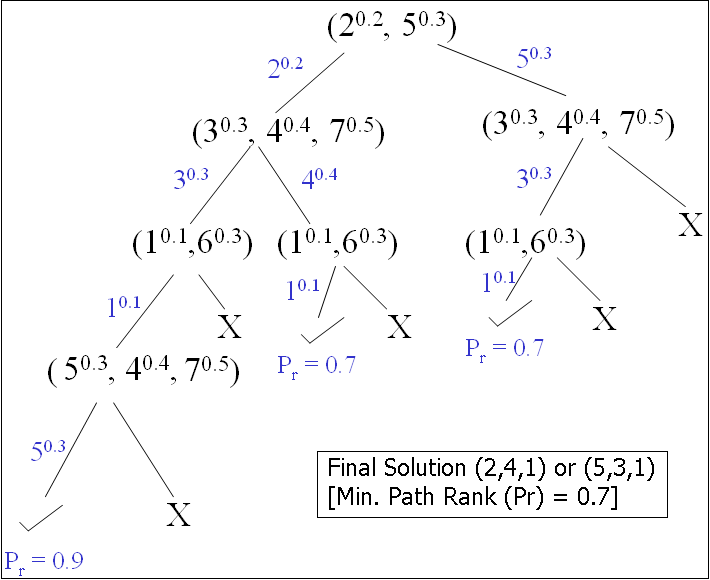
\includegraphics[width=90mm]{Figures/fig1.png}
			\caption{Giải thuật HST được chỉnh sửa dựa theo thứ hạng của phát biểu \label{overflow}}
		\end{figure}
		
		\hspace*{.05\textwidth} Như được thể hiện trong hình, bằng cách chọn phát biểu có hạng thấp nhất trong từng tập trong khi xây cạnh của HST, giải thuật chỉ tạo ra 3 hitting sets, 2 trong số đó tối tiểu, trong khi hạn chế được một số lượng lớn số lần kiểm tra đường đi, (thể hiện bằng \xmark). Giải pháp sửa lỗi được tìm ra trong tập có $P_{r}$ nhỏ nhất là {2,4,1} hoặc {5,3,1}.
		
		\hspace*{.05\textwidth} Tuy vậy, có một hạn chế khi sử dụng quy trình vừa nêu trên để tạo ra kế hoạch sửa lỗi, như phân tích tác động ngữ nghĩa của phát biểu chỉ được thực hiện ở cấp độ là một phát biểu đơn lẻ, trong khi một loạt tác động khác chưa được tính tới mỗi lần một HS được tìm thấy. Điều này có thể dẫn tới một giải pháp kém tối ưu. Ví dụ:
		\begin{enumerate}
			\item	DisjointClasses(Car Plane Ship)
			\item	EquivalentClass(FlyingCar (Car and Plane))			
		\end{enumerate}
		Trong ví dụ trên, bỏ \texttt{Plane} ra khỏi phát biểu (1) sẽ hạn chế mất mát về nghĩa hơn là xóa hết cả phát biểu (1), vì có thể disjoint giữa Car và Ship có thể được sử dụng đâu đó trong ontology mà chưa được tính đến.
		\hspace*{.05\textwidth} Để khắc phục hạn chế này, một chỉnh sửa khác được đưa ra là cứ mỗi lần tìm ra hitting-set(HS), chúng ta sẽ tính lại thứ hạng của đường đi (path-rank) cho HS dựa trên một loạt tác động của các phát biểu trong hitting-set. Giải thuật bây giờ sẽ tìm được giải pháp tối thiểu được path-ranks mới.
		\\
		Trên đây là ý tưởng cơ bản của giải thuật HST, ngoài ta còn những mục về cải thiện các giải pháp sửa lỗi và gợi ý các phát biểu sửa lỗi xin đọc thêm ở \cite{repair}.
		
		\subsection{Ứng dụng HST để xác định tất cả giải thích cho kết quả suy luận\cite{matt_horridge}}
		Ngoài ứng dụng vừa được đề cập ở trên, Hitting Set Tree còn được áp dụng để tìm tất cả các giải thích cho một kết quả suy luận, giống như một trong chức năng chính của Axiom Pinpointing Service được đề cập lúc nãy. Tuy nhiên, không giống như khái niệm HST của Reiter vừa được giới thiệu ở trên, ở đây chúng ta sẽ có HST với quy ước như sau.
		
		\hspace*{.05\textwidth} Với ontology $\beta$ $\models$ $\eta$, một cây hitting set (HST) cho $\eta$ trong $\beta$ là một cây hữu hạn, bao gồm node được dán nhãn bằng các kiểm chứng (justifications) hay các phát biểu chứng minh $\beta$ $\models$ $\eta$ và cạnh được đánh dấu với phát biểu trong $\beta$. Từng non-leaf(không phải lá) node $v$ nối với một node kế cận $v^{'}$ qua một cạnh được dán nhãn với một phát biểu $\alpha$ với $\alpha$ nẳm trong nhãn của $v$, nhưng không nằm trong nhãn của $v^{'}$. Nhãn của $v^{'}$ có thể là một tập hợp rỗng, trong trường hợp đó $v^{'}$ phải là node lá (leaf node). Ngoài ra, với bất kì node $v^{''}$, tập chứa các phát biểu dán nhãn cho đường đi từ $v^{''}$ tới gốc cây (tree root) \textit{không} giao với kiếm chứng(hay các phát biểu chứng minh) dán nhãn $v^{''}$.
		
		\hspace*{.05\textwidth} Quá trình xây dựng HST có thể được thực hiện bằng các giải thuật \textit{breadth first} hay \textit{depth first}. Dù được sử dụng theo cách nào, các nguyên lý và các luật để tạo và dán nhãn cạnh, node trên cây đều như nhau. Khi mở rộng cây từ node $v$ đến một node mới $v^{'}$ quy trình cơ bản đều diễn ra như sau:
		\begin{enumerate}
			\item Chọn một phát biểu $\alpha$ nằm trong nhãn của $v$ nhưng không dán nhãn một cạnh nối $v$ tới bất kì node kế cận nào.
			\item Gọi $S$ là hội của (union of) {$\alpha$} và tập những phát biểu nằm trên cạnh, tạo thành đường đi từ $v$ tới root node. Loại bỏ $S$ khỏi $\beta$ ta được $\beta^{'}$.
			\item Nếu $\eta$ thỏa $\beta^{'}$ $\models$ $\eta$ thì tìm một kiểm chứng (justification) $J$ cho $\eta$ trong $\beta^{'}$. Nếu $\beta^{'}$ $\not\models$ $\eta$ thì gán $J$ = $\emptyset$.
			\item Tạo một node mới $v^{'}$ và dán nhãn cho $v^{'}$ bằng tập $J$ ở bước trên.
			\item Tiếp tục mở rộng HST theo một hướng bằng cạnh $e$ = ($v$, $v^{'}$) tương tự như bước 1 cho tới khi không tìm được tập $J$ = $\emptyset$ như ở bước 2.
			\item Đưa các phát biểu trong $S$ trở lại $\beta$.
		\end{enumerate}
		Ví dụ sau mô tả lại quy trình trên, cho ontology $\beta$  với các phát biểu sau:
		\begin{enumerate}
			\item $A$ $\subseteq$ $B$
			\item $B$ $\subseteq$ $D$ 
			\item $A$ $\subseteq$ $\exists$ $R.C$ 
			\item $\exists$ $R.\top$ $\subseteq$ $D$
		\end{enumerate} 
		
		Trong đó $\eta$ $=$ $A\subseteq$ $D$. HST cho $\beta$ $\models$ $A$ $subseteq$ $D$ được thể hiện ở hình 2.2. Bắt đầu di chuyển tại root node, node được dán nhãn bởi $J_{1}$\textsuperscript{*}, mở rộng HST về phía bên trái bằng cách chọn phát biểu $A\subseteq$ $B$ trong $J_{1}$ với điều kiện $A\subseteq$ $B$ chưa dán nhãn bất kì cạnh nào nối với root node sau đó loại bỏ phát biểu $A\subseteq$ $B$ khỏi $\beta$ và tính toán lại kiếm chứng (justifications) thỏa $\langle\beta$ $\backslash$ $\{A\subseteq$ $B\}\rangle$ $\models$ $A\subseteq$ $D$. Trong trường hợp này, chúng ta tìm được kiểm chứng $J_{2}$ trong $\beta$ $\backslash$ $\{A\subseteq$ $B\}$, giải thích được tại sao $A\subseteq$ $D$. Tiếp tục đi về phía bên trái của node $J_{2}$, chọn $A\subseteq$ $\exists$ $R.C$ trong $J_{2}$ tương tự cách chọn ở bước 1. Sau đó tìm kiếm các kiểm chứng trong $\beta^{'}$ $\equiv$ $\beta$ $\backslash$ $\{A\subseteq$ $\exists$ $R.C$, $A\subseteq$ $B\}$, kết quả là chúng ta không tìm được kiểm chứng trong $\beta^{'}$ giải thích cho $A\subseteq$ $D$ hay có thể nói là $\beta^{'}$ $\not\models$ ($A\subseteq$ $D$), do vậy node kế tiếp được dán nhãn bằng $\emptyset$ vì lúc này $J$ $=$ $\emptyset$ (bước 3). Mỗi lần như vậy ta tìm ra leaf-node, chúng ta sẽ đưa $S$ trở lại $\beta$ và bắt đầu lại quá trình tìm kiếm.
		\begin{figure}[ht!]
			\centering
			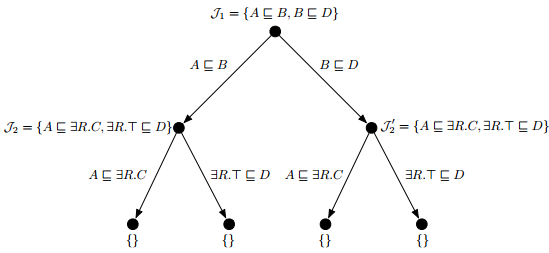
\includegraphics[width=110mm]{Figures/fig2.png}
			\caption{Hitting Set Tree dùng để tìm kiếm kiểm chứng \label{overflow}}
		\end{figure}
		% A foot note
		{\let\thefootnote\relax\footnotetext{*\textit{
					$J_{1}$,$J_{2}$,$J_{2}^{'}$ được tính ra nhờ giải thuật Black-box hoặc Glass-box được đề cập ở trên.
				}}
				\hspace*{.05\textwidth} Quá trình lặp lại cho đến khi chúng ta không còn tạo được node mới nào, tại thời điểm này thì việc xây dựng HST cũng hoàn tất. \textit{Tất cả} các kiểm chứng để giả thích cho $\beta$ $\models$ $\eta$ chính là nhãn của các node trong HST. Thêm một điều nữa, là tất cả các đặc điểm đơn giản nhất để chứng minh $\beta$ $\models$ $\eta$ nằm trên các cạnh từ leaf-node tới root-node của cây.
				\\
				Ví dụ vừa nếu trên chỉ biểu diễn những bước cơ bản nhất để xây dựng một HST nhưng quan tâm đến bất kì khả năng tối ưu hóa nào cho giải thuật. Để đạt được một hiệu năng chấp nhận được khi ứng dụng trong thực tế thì 2 giải pháp tối ưu sẽ được nêu ra sau đây.
				
				\paragraph{Early Path Termination} - Trong phiên bản chưa tối ưu ở trên, một node $n$ bất kì khi tạo cạnh mới với phát biểu thuộc tập $H(n)$, với $H(n)$ là tập phát biểu dán nhãn $n$, phát biểu trên cạnh mới này không được nằm trên bất kì cạnh nào nối $n$ với một node kế cận (successor nodes). Chúng ta gọi các nodes có khả năng mở rộng (tạo được cạnh mới) là \textit{open} nodes, ngược lại các leaf-nodes không có khả năng mở rộng là \textit{closed} nodes,. Để thực hiện tối ưu hóa, sẽ có trường hợp mà những nodes không phải leaf-nodes có thể được dán nhãn bởi những tập khác $\emptyset$ những vẫn sẽ được đánh dấu là \textit{closed} nodes. Trong tình huống này, đường đi từ \textit{closed} node tới root được chỉ định là \textit{early termination} - kết thúc sớm. Để phát hiện được \textit{early termination} chúng ta sẽ làm theo quy trình sau: Nếu một HST $T$ chứa một open node $v_{1}$, có đường đi $P_{1}$ tới root node, có thêm một open node $v_{2}$ cũng trong $T$, có đường tới root node là $P_{2}$. Nếu tập dán nhãn cho $P_{1}$ bằng với tập dán nhãn cho $P_{2}$ thì $v_{2}$ sẽ được đánh dấu là \textit{closed} node và không cần thiết phải mở rộng thêm nữa. Ví dụ chúng ta có ontology $O$ chứa các phát biểu sau $O=\{1, 2, 3, 4, 5\}$ và $O$ $\models$ $\alpha$
				\begin{figure}[ht!]
					\centering
					\begin{tikzpicture}[every tree node/.style={draw,circle},
					level distance=1.25cm,sibling distance=1cm,
					edge from parent path={(\tikzparentnode) -- (\tikzchildnode)}]
					\Tree
					[.1,2
					\edge node[auto=right,pos=.6] {$1$};
					[.2,3,5 
					\edge node[auto=right,pos=.8] {$2$};
					[.3,5 
					\edge node[auto=right,pos=.8] {$3$};
					[.{$\{\}$} ]
					\edge node[auto=right,pos=.8] {$5$};
					[.{$\{\}$} ]    	
					]
					\edge node[auto=left,pos=.8] {$3$};
					[.{$\{\}$} ]
					\edge node[auto=left,pos=.8] {$4$};
					[.{$\{\}$} ]
					]
					\edge node[auto=left,pos=.6] {$2$};
					[.1,3,4
					\edge node[auto=right,pos=.8] {$1$};
					[.X ]
					\edge node[auto=left,pos=.8] {$3$};
					[.{$\{\}$} ]
					]
					]
					\end{tikzpicture}
					\caption{Early Termination trong HST Explanation \label{overflow}}
				\end{figure}
				
				Chúng ta bắt đầu di chuyển root node với tập $\{1,2\}$ là các phát biểu đầu tiên tìm được trong $O$ chứng minh được $O$ $\models$ $\alpha$, thực hiện tương tự các bước đã được miêu tả ở trên ta thu được node $\{3,5\}$ là các phát biểu giải thích cho $O$ $\models$ $\alpha$, tới lúc này ta có thể thấy tập chứ đường đi theo cạnh từ node $\{3,5\}$ tới root node là $P_{1}=\{2,1\}$. Nhìn về phía bên phải ta phát hiện khi mở rộng cạnh từ node $\{1,3,4\}$ ta thu được đường đi về root node là $P_{2}=\{1,2\}$, ta thấy $P_{1} \equiv P_{2}$ do vậy nên khi dán nhãn cho node kế tiếp (được đánh dâu \xmark cho \textit{closed} node) chúng ta sẽ bỏ $\{1,2\}$ khỏi $O$ để được $O^{'}=\{3,4,5\}$, sẽ có một node giống y như node $\{3,5\}$ sẽ xuất hiện lần nữa ở node kế tiếp này nên việc kết thúc ở đây là cần thiết vì chúng ta sẽ tiếp kiệm được việc kiểm tra lại $\{3,5\}$ như ở bên trái.
				
				\paragraph{Justification Reuse} - Cách quan trọng thứ hai để tối ưu là sử dụng lại các kiểm chứng. Trong phiên bản không tối ưu sử dụng ở ví dụ ontology $\beta$ ở trên, kiểm chứng được tìm ra nhờ các giải thuật Blackbox hay Glassbox cho từng node $v$ được thêm vào cây. Kiểm chứng hay tập các phát biểu được sử dụng để dán nhãn $v$, được tính toán dựa trên $O \backslash S$, với $S$ là tập các nhãn trên đường đi từ $v$ về root node. Thay vì dùng Glassbox hay Blackbox để tính $J$ trong $O \backslash S$, chúng ta có thể làm theo cách sau: nếu HST chứa vài node khác $v^{'}$ mà được dán nhãn với kiểm chứng $J$, và $S$ không giao (có phần tử chung) với $J$ thì $J$ có thể được sử dụng làm nhãn cho $v$. Lý do là vì khi $J\subseteq$ $O$ và $S\cap J = \emptyset$ thì sẽ tồn tại trường hợp $J\subseteq O \backslash S$, từ đó $J$ được tính như một kiểm chứng cho để có thể dán nhãn $v$. Sử dụng lại các phát biểu chứng minh (hay kiểm chứng) sẽ giúp tiết kiệm nhiều lời gọi hàm không cần thiết tới Blackbox hoặc Glassbox từ đó tăng được hiệu năng.
				\\
				\paragraph{Kết luận} Tính năng vừa trình bày \textit{Tìm tất cả các giải thích cho kết quả suy luận}, kĩ thuật \textit{Axiom Pinpoint} và \textit{BlackBox} được đã được áp dụng trong thư viện lập trình OWL-API \cite{owlapi} sẽ được chúng em giới thiệu trong chương tiếp theo.
